\chapter*{Annexure A: Criteria 1 Supporting Documents}
\addcontentsline{toc}{chapter}{Annexure A: Criteria 1 Supporting Documents}
\label{app:crtieria-1}

Here we provide supporting annexures required for the Criterion 1 i.e. Program Educational Objectives (PEOs).

\setcounter{section}{0}
\renewcommand{\thesection}{A.\arabic{section}}
\section{Legacy Survey Forms}
\label{app:legacy forms}
The full Employer and Alumni legacy survey forms referenced in Criterion~1 are reproduced below exactly as administered:

\setcounter{figure}{0}
\renewcommand{\thefigure}{A.\arabic{figure}}
\begin{figure}[!h]
\centering
\fbox{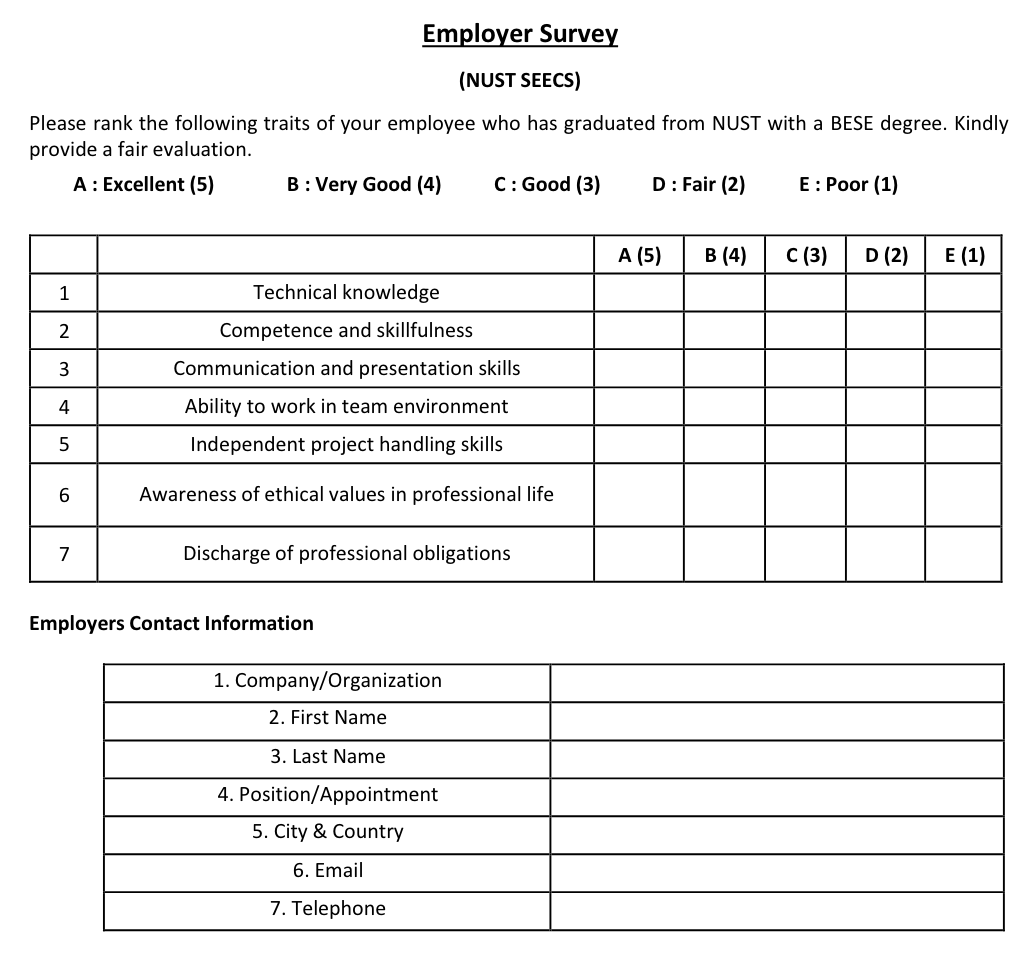
\includegraphics[width=1.0\textwidth]{images/front_matter/media/legacy employer form.png}}
\caption{Legacy Employer Survey Form}
\label{fig:legacy employer form}
\end{figure}

\begin{figure}[!h]
\centering
\fbox{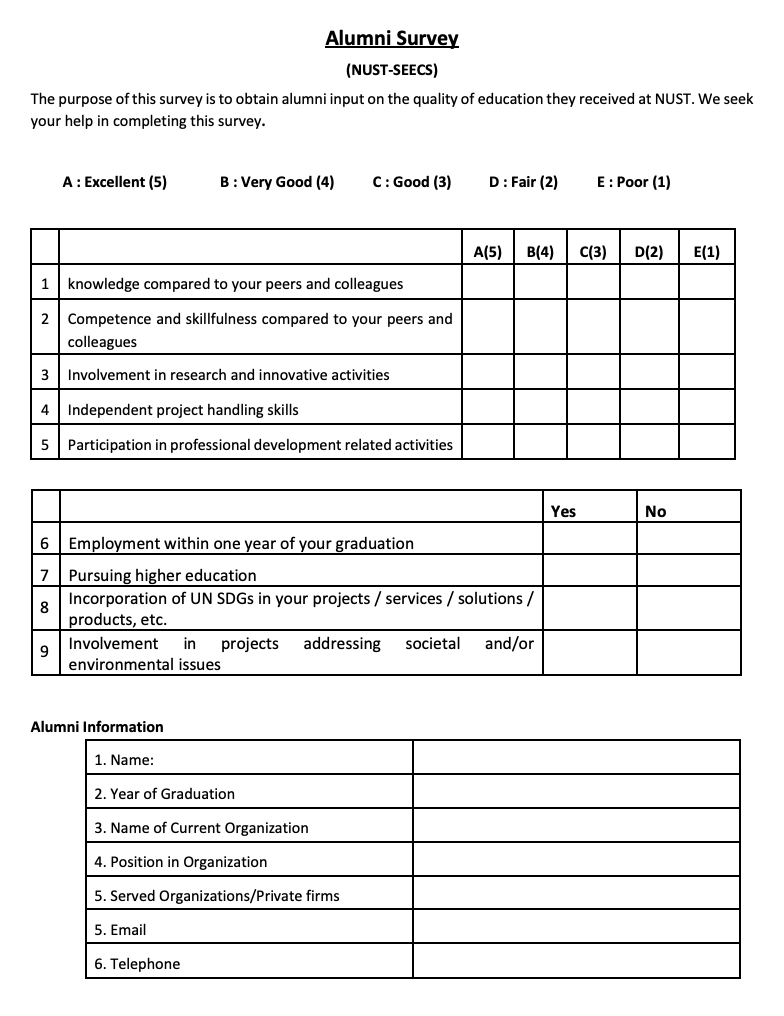
\includegraphics[width=1.0\textwidth]{appendices/criterion_1/legacy alumni form.png}}
\caption{Legacy Alumni Survey Form}
\label{fig:legacy alumni form}
\end{figure}

\section{Legacy PEO Evaluation System and Results (Pre-2026)}\label{app:legacy_peo_evaluation}

This annexure describes the evaluation mechanism and attainment results of the legacy PEO evaluation system, referenced in Criterion~1. 

\subsection{Legacy Evaluation Mechanism}

Under the legacy system, each PEO was assessed through a set of Key Performance Indicators (KPIs) derived from annual Alumni and Employer surveys. Indicator design accounted for diversity in graduate career paths e.g., employment, entrepreneurship, or higher education, so that a graduate's choice of path did not itself count against attainment. Each KPI was expressed as the percentage of respondents responding favourably to a specific survey item, with an attainment threshold of 50\% or 60\% depending on the indicator. A PEO was considered attained only if all of its constituent sub-KPIs individually met their respective thresholds, with cumulative PEO attainment computed as the equal-weight average of its sub-KPIs. Following KPIs were defined in the old scheme.

\noindent\textbf{PEO 1 --- Demonstrate sound software engineering knowledge and skill set.}
\begin{itemize}[leftmargin=1.5em,topsep=2pt]
\item 60\% of respondent employers are satisfied with technical knowledge of employed graduates.
\item 60\% of respondent employers are satisfied with competence and skills of employed graduates.
\item 60\% of respondent graduates gave positive feedback on their knowledge compared to their peers.
\item 60\% of respondent graduates gave positive feedback on their competence compared to their peers.
\item 50\% of respondent graduates are employed within one year of their graduation.
\item 50\% of respondent graduates are pursuing higher education.
\end{itemize}

\noindent\textbf{PEO 2 --- Lead diverse teams and work collaboratively to develop innovative solutions.}
\begin{itemize}[leftmargin=1.5em,topsep=2pt]
\item 60\% of respondent employers are satisfied with the communications skills of employed graduates.
\item 60\% of respondent employers are satisfied with the teamwork skills of employed graduates.
\item 60\% of respondent employers are satisfied with the independent project handling skills of employed graduates.
\item 60\% of respondent graduates are involved in research and/or innovation activities.
\item 60\% of respondent graduates have handled projects independently.
\item 50\% of respondent graduates are involved in professional development activities.
\end{itemize}

\noindent\textbf{PEO 3 --- Conduct professional practice for sustainable development with due consideration for societal, ethical, and environmental aspects.}
\begin{itemize}[leftmargin=1.5em,topsep=2pt]
\item 60\% of respondent employers are satisfied with adherence to ethical values by employed graduates.
\item 60\% of respondent employers are satisfied with the discharge of professional obligations of employed graduates.
\item 50\% of respondent graduates have incorporated UN SDGs in their projects / services / solutions / products etc.
\item 50\% of respondent graduates are involved in projects addressing societal and/or environmental issues.
\end{itemize}

\subsection{Legacy Evaluation Results (2025)}

Table~\ref{tab:legacy_results} presents the attainment results obtained under the legacy evaluation system, using Alumni and Employer survey data collected in 2025.
\setcounter{table}{0}
\renewcommand{\thetable}{A.\arabic{table}}
\begingroup
\scriptsize
\setlength{\tabcolsep}{4pt}
\renewcommand{\arraystretch}{1.2}
\begin{longtable}[]{@{}>{\raggedright\arraybackslash}p{0.06\textwidth}>{\raggedright\arraybackslash}p{0.52\textwidth}>{\raggedright\arraybackslash}p{0.20\textwidth}>{\centering\arraybackslash}p{0.10\textwidth}@{}}
\caption{Attainment of PEOs under the Legacy Evaluation System (Alumni/Employer surveys, data collected in 2025)}\label{tab:legacy_results}\\
\toprule
\multicolumn{4}{@{}>{\raggedright\arraybackslash}p{0.92\textwidth}@{}}{\textbf{PEO 1}: Demonstrate sound software engineering knowledge and skill set.}\\
\midrule
\textbf{S. No.} & \textbf{KPI} & \textbf{Measurement Tool} & \textbf{Attainment \%}\\
\midrule
\endfirsthead
\toprule
\textbf{S. No.} & \textbf{KPI} & \textbf{Measurement Tool} & \textbf{Attainment \%}\\
\midrule
\endhead
1 & 60\% of respondent employers are satisfied with technical knowledge of employed graduates & Employer Survey (Q1) & 85\%\\
2 & 60\% of respondent employers are satisfied with competence and skills of employed graduates & Employer Survey (Q2) & 86\%\\
3 & 60\% of respondent graduates gave positive feedback on their knowledge compared to their peers & Alumni Survey (Q1) & 76\%\\
4 & 60\% of respondent graduates gave positive feedback on their competence compared to their peers & Alumni Survey (Q2) & 76\%\\
5 & 50\% of respondent graduates are employed within one year of their graduation & Alumni Survey (Q6) & 89\%\\
6 & 50\% of respondent graduates are pursuing higher education & Alumni Survey (Q7) & 36\%\\
\addlinespace
\midrule
\multicolumn{4}{@{}>{\raggedright\arraybackslash}p{0.92\textwidth}@{}}{\textbf{PEO 2}: Lead diverse teams and work collaboratively to develop innovative solutions.}\\
\midrule
\textbf{S. No.} & \textbf{KPI} & \textbf{Measurement Tool} & \textbf{Attainment \%}\\
\midrule
1 & 60\% of respondent employers are satisfied with the communications skills of employed graduates & Employer Survey (Q3) & 84\%\\
2 & 60\% of respondent employers are satisfied with the teamwork skills of employed graduates. & Employer Survey (Q4) & 85\%\\
3 & 60\% of respondent employers are satisfied with the independent project handling skills of employed graduates & Employer Survey (Q5) & 81\%\\
4 & 60\% of respondent graduates are involved in research and/or innovation activities & Alumni Survey (Q3) & 69\%\\
5 & 60\% of respondent graduates have handled projects independently & Alumni Survey (Q4) & 79\%\\
6 & 50\% of respondent graduates are involved in professional development activities & Alumni Survey (Q5) & 76\%\\
\addlinespace
\midrule
\multicolumn{4}{@{}>{\raggedright\arraybackslash}p{0.92\textwidth}@{}}{\textbf{PEO 3}: Conduct professional practice for sustainable development with due consideration for societal, ethical, and environmental aspects.}\\
\midrule
\textbf{S. No.} & \textbf{KPI} & \textbf{Measurement Tool} & \textbf{Attainment \%}\\
\midrule
1 & 60\% of respondent employers are satisfied with adherence to ethical values by employed graduates. & Employer Survey (Q6) & 86\%\\
2 & 60\% of respondent employers are satisfied with the discharge of professional obligations of employed graduates. & Employer Survey (Q7) & 78\%\\
3 & 50\% of respondent graduates have incorporated UN SDGs in their projects / services / solutions / products etc. & Alumni Survey (Q8) & 52\%\\
4 & 50\% of respondent graduates are involved in projects addressing societal and/or environmental issues. & Alumni Survey (Q9) & 64\%\\
\bottomrule
\end{longtable}
\endgroup

Under the legacy criterion requiring every sub-KPI to meet its threshold individually, PEO~2 and PEO~3 were fully attained. For PEO~1, five of the six sub-KPIs exceeded their thresholds. The indicator measuring the proportion of graduates pursuing higher education reached 36\% against a 50\% threshold. On an equal-weight cumulative basis, the attainment levels were approximately 75\%, 79\%, and 70\% for PEO~1, PEO~2, and PEO~3, respectively. 

Figure~\ref{fig:legacy_analysis} shows the per-KPI attainment for each PEO under the legacy evaluation system, with the dashed line in each panel indicating the applicable attainment threshold (50\% or 60\%, depending on the indicator). All indicators meet their respective thresholds except PEO~1 KPI-6 (pursuing higher education), which falls below its 50\% threshold.

\begin{figure}[tb]
\centering
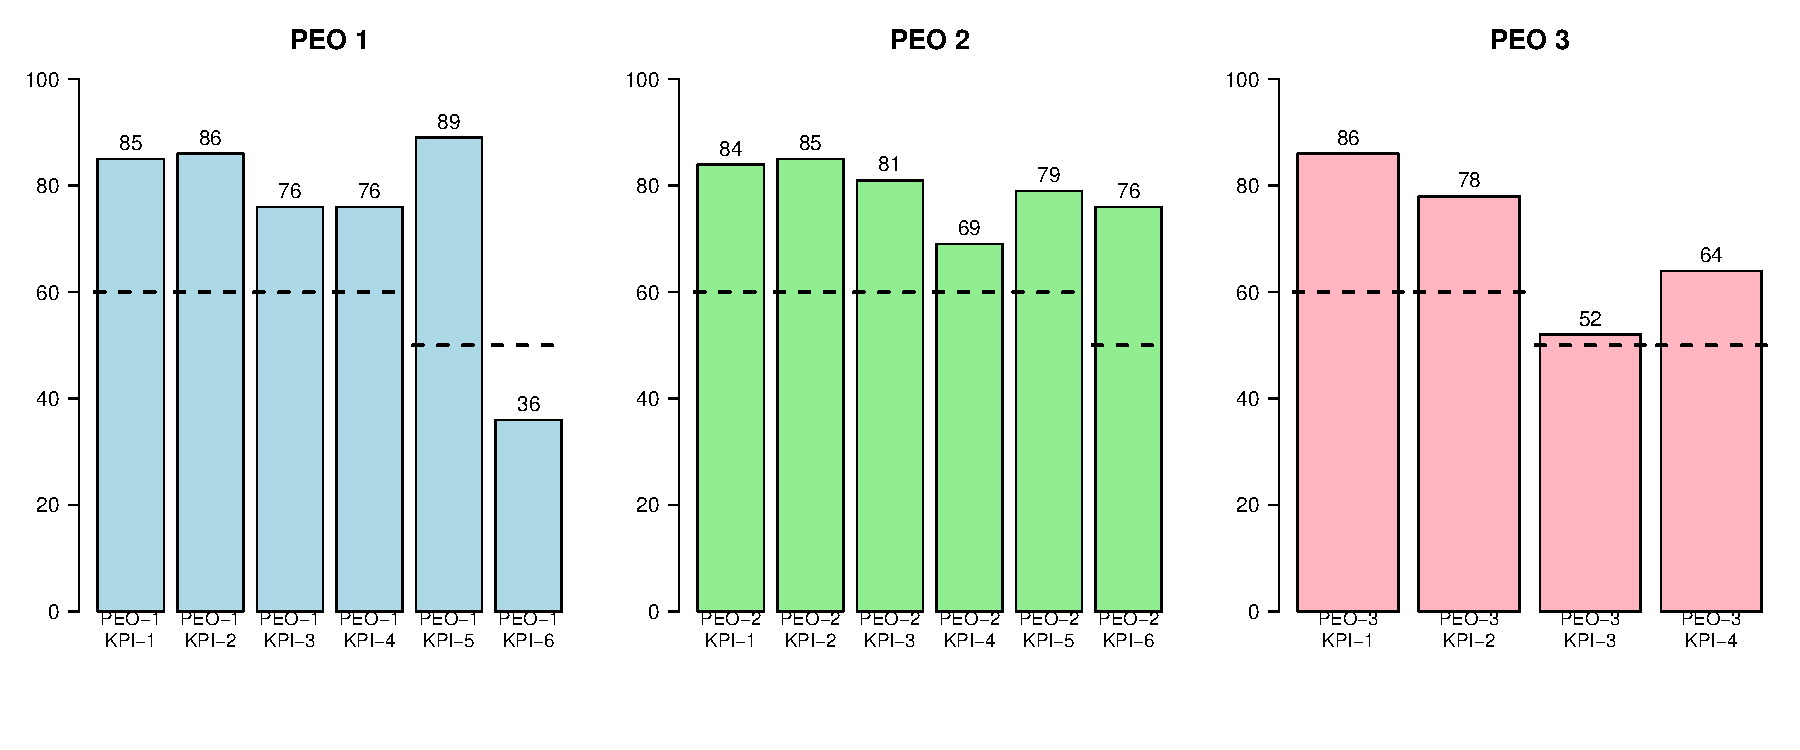
\includegraphics[width=\textwidth]{images/criterion_1/media/legacy_analysis.pdf}
\caption{Per-KPI attainment under the Legacy Evaluation System (data collected in 2025). The dashed line in each panel marks the applicable attainment threshold for that indicator.}
\label{fig:legacy_analysis}
\end{figure}

The single below-threshold indicator reflects a structural limitation of the legacy instrument rather than a shortfall in program outcomes. Pursuit of higher education is a binary indicator that does not, on its own, represent PEO attainment, since graduates who enter employment instead of higher education are not demonstrating a deficiency against the objective. Limitations of this nature where indicators are only loosely aligned with PEO-level outcomes, together with a rigid all-or-nothing pass rule, motivated the revised evaluation system described in Criterion~1.

\section{IAB Feedback: Full Closed-Loop and Open Recommendation Records}\label{app:iab_feedback_full}

This annexure reproduces, in full, the two IAB feedback tables summarized in Criterion~1. The complete closed-loop record of feedback items with documented evidence of implementation, and the complete list of standing/open recommendations, restricted to items sourced from IAB sessions held in 2024 or later, with one exception, i.e. the 13th November 2023 session is retained below because it is the documented origin of the Revised (2026) PEO Evaluation System, the report's principal CQI action (Section~\ref{attainment-of-peos}). The official minutes underlying these entries, including the 13th November 2023 session, are reproduced in Appendix~\ref{app:iab_minutes} and evidence folder.

\subsection{Closed-Loop Actions: Feedback Implemented and Verified (Full Record)}

\begingroup
\footnotesize
\setlength{\tabcolsep}{4pt}
\renewcommand{\arraystretch}{1.2}
\begin{longtable}[]{@{}>{\raggedright\arraybackslash}p{0.28\textwidth}>{\raggedright\arraybackslash}p{0.18\textwidth}>{\raggedright\arraybackslash}p{0.46\textwidth}@{}}
\caption{Closed-Loop IAB Feedback and Actions Taken (2023 origin item retained, otherwise 2025)}\label{tab:iab_closed_loop}\\
\toprule
\textbf{Industry Feedback} & \textbf{Source / Date} & \textbf{Action Taken}\\
\midrule
\endfirsthead
\toprule
\textbf{Industry Feedback} & \textbf{Source / Date} & \textbf{Action Taken}\\
\midrule
\endhead
\midrule
\multicolumn{3}{r}{\footnotesize\itshape Continued on next page}\\
\endfoot
\bottomrule
\endlastfoot
Alumni Survey item (Q5) was found to inadequately assess PEO-2 attainment. & IAB Meeting, 13th November 2023 & As recorded in the minutes (ref:Detailed minutes evidence folder ), the item was relocated to PEO-3, where it aligns with the corresponding KPI, endorsed in the same session.\\
\addlinespace
PEC observation (2023 Accreditation Visit): Lack of correlation in the survey forms used to assess certain PEO-2/PEO-3 sub-KPIs, reinforced by the IAB's concern over Alumni Survey Q5 (see above). & PEC Accreditation Visit, 2023, reiterated IAB Meeting, 13th November 2023 & The Alumni and Employer Survey instruments were fully redesigned, with items mapped directly to PEOs, as the Revised (2026) Evaluation System. The revised forms were reviewed and approved by the SE Departmental Board of Studies (DBS) on 20th April 2026. These were presented to and ratified by the SEECS HoDs' forum and the Faculty Board of Studies (FBS) of 21st April 2026, and finally presented to and endorsed by the IAB on 5th May 2026. The approved forms were then circulated by email to Alumni and Employers for input and used at the department's Open House in May 2026.\\
\addlinespace
Introduce a Quantum Computing course. & IAB Meeting, 28th February 2025 (CEO, Emumba) & A dedicated elective, ``Introduction to Quantum Computing'' (offered in 3+1 and 2+1 credit-hour variants, covering superposition, entanglement, quantum algorithms, and hands-on labs using Qiskit-based simulators), was proposed via a SEECS-wide working paper (sponsored by SEECS, not the SE department alone) for inclusion as an elective in the BESE (Software Engineering), BSCS, BSAI, and BSDS curricula. The working paper records the course as approved by the DBS, for introduction from Spring 2026.\\
\addlinespace
Enable cross-departmental minor courses (e.g., SEECS students taking courses at NBS). & IAB Meeting, 28th February 2025 & Already available under NUST's University-wide Minors policy: SEECS students including (Software Engineering) may register for the Management minor at NUST Business School (NBS), subject to a minimum CGPA of 2.75, while SEECS reciprocally offers minors in Software Engineering, Computer Science, Data Science, and Artificial Intelligence to students of other NUST institutions (NUST Undergraduate Student Handbook, 28th August 2024 edition, Chapter 6, Para 2 ``Option of Minors'').\footnote{National University of Sciences and Technology, \textit{Undergraduate Student Handbook}, 28th August 2024 edition, Chapter 6, Para 2. Available at \url{https://seecs.nust.edu.pk/wp-content/uploads/2024/09/28-Aug-2024-Undergraduate-Handbook.pdf}.}\\
\addlinespace
Consider open-book examination formats. & IAB Meeting, 28th February 2025 (ITnIS Consulting) & Already available under existing NUST examination policy: the concerned faculty/invigilator may announce, in advance of a quiz, OHT, or mid/end-semester examination, the books, notes, or other material students may refer to during the test, effectively enabling an open-book format at faculty discretion (NUST Undergraduate Student Handbook, 28th August 2024 edition, Chapter 2, Para 8 ``Use of Reference Material during Test/Examination'').\footnote{National University of Sciences and Technology, \textit{Undergraduate Student Handbook}, 28th August 2024 edition, Chapter 2, Para 8. Available at \url{https://seecs.nust.edu.pk/wp-content/uploads/2024/09/28-Aug-2024-Undergraduate-Handbook.pdf}.}\\
%\addlinespace
%Introduce certification-style courses. & IAB Meeting, 28th February 2025 (ITnIS Consulting) & NUST recently approved 1–3 CH range (per WP No. 2, 73rd ACM, 9th February 2026, in consistence with HEC's CS/IT-specific elective-replacement provision (Letter HEC/CURR/GEN/2025/8036, 15th September 2025, Annex-A, Para 5), but differs from PEC's own proposal of a broader 6–12 CH range floated at its Task Force's inaugural meeting of 21st May 2025 and subsequently circulated for institutional input via Letter PEC/EAD/EQEEP/2025/04 (14th July 2025). That proposal remains subject to ratification by PEC's Engineering Accreditation Board (EAB) and Governing Body and has not yet been issued as a final SOP. The department intends to therefore adopt NUST policy in line with the more specific and more recent HEC guidance while awaiting PEC's final mechanism, and will revise credit-hour equivalencies if required once PEC's SOP is issued.\\
\end{longtable}
\endgroup

\subsection{Standing and Emerging Recommendations (Full Record)}

\begingroup
\footnotesize
\setlength{\tabcolsep}{4pt}
\renewcommand{\arraystretch}{1.2}
\begin{longtable}[]{@{}>{\raggedright\arraybackslash}p{0.68\textwidth}>{\raggedright\arraybackslash}p{0.24\textwidth}@{}}
\caption{Open IAB Recommendations Pending Implementation}\label{tab:iab_open}\\
\toprule
\textbf{Recommendation (Not Yet Closed)} & \textbf{Source / Date}\\
\midrule
\endfirsthead
\toprule
\textbf{Recommendation (Not Yet Closed)} & \textbf{Source / Date}\\
\midrule
\endhead
\midrule
\multicolumn{2}{r}{\footnotesize\itshape Continued on next page}\\
\endfoot
\bottomrule
\endlastfoot
Expand coverage of AI agents, reverse engineering, and data-science algorithms. & IAB Meeting, 28th February 2025 (CEO, Emumba)\\
Establish a faculty ``boot camp'' to close the skills gap between academia and industry practice, targeted at PhD/MS scholars. & IAB Meeting, 7th May 2025, recorded as Action Point 2\\
Broaden ``Applied AI in Education'' into a cross-sector applied-AI offering. Split DevOps and Machine Learning into separate courses. & IAB Meeting, 7th May 2025, recorded as Action Point 1\\
Formalise a mentorship partnership (e.g., with Novatec X) to provide affordable, industry-led mentorship to students and researchers. & IAB Meeting, 7th May 2025, recorded as Action Point 3\\
Improve student and faculty access to premium cloud/AI tools to maximise use of available cloud-credit programmes. & IAB Meeting, 7th May 2025, recorded as Action Point 4\\
Increase the number of internship placements and recruitment drives connected to Open House events. & IAB Meeting, 28th February 2025\\
Continue to strengthen graduate soft skills, communication, customer orientation, and professional ethics, a recurring, sustained industry request across multiple sessions. & IAB Meetings: 2nd May 2024, 28th February 2025, 5th May 2026\\
\end{longtable}
\endgroup
%%%%%%%%%%%%%%%%%%%%%%%%%%%%%%%%%%%

\section{IAB Meeting Minutes (2023 Origin Session, and 2024--2026)}\label{app:iab_minutes}

The original minutes of the selected few relevent Industry Advisory Board (IAB) sessions cited in Criterion~1 are reproduced below exactly as recorded. Details of each IAB proceeding with each session presented will be provided in evidence folder at the time of visit.

\begin{figure}[!h]
\centering
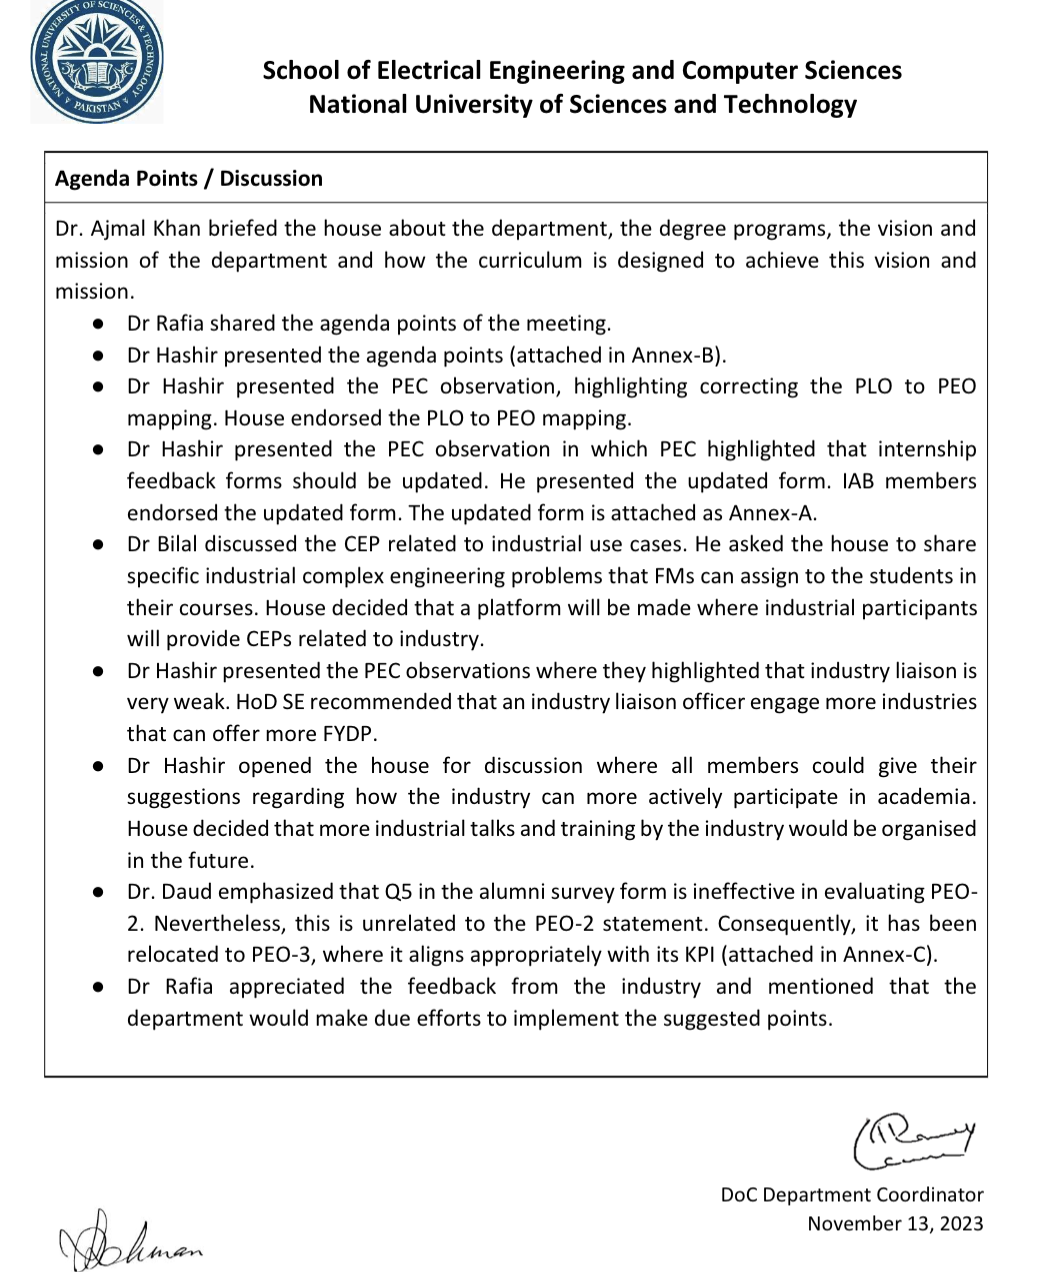
\includegraphics[width=0.8\textwidth]{appendices/criterion_1/IAB 2023.png}
\caption{IAB Meeting Minutes 13th November 2023}
\label{fig:iab 2023}
\end{figure}

The meeting on 13th November 2023 was attended by following faculty and industry representatives.

\begin{figure}[!h]
\centering
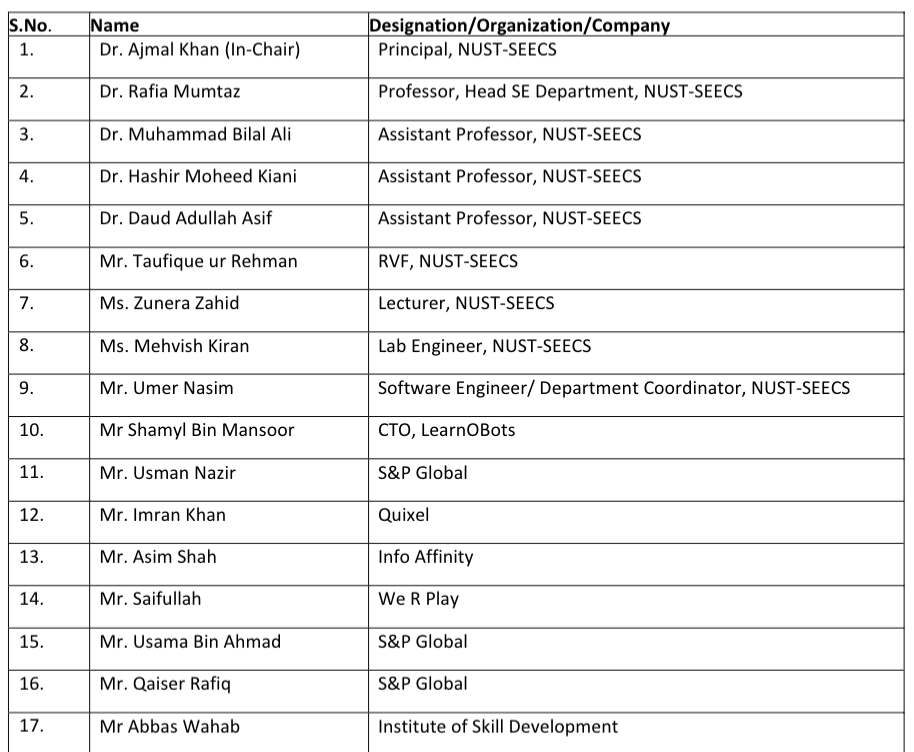
\includegraphics[width=0.79\textwidth]{appendices/criterion_1/iab 2023 attendance.png}
\caption{IAB Meeting Participants 13th November 2023}
\label{fig:iab 2023 attendees}
\end{figure}

The subsequent IAB meeting was held on 2nd May 2024. 

\begin{figure}[!h]
\centering
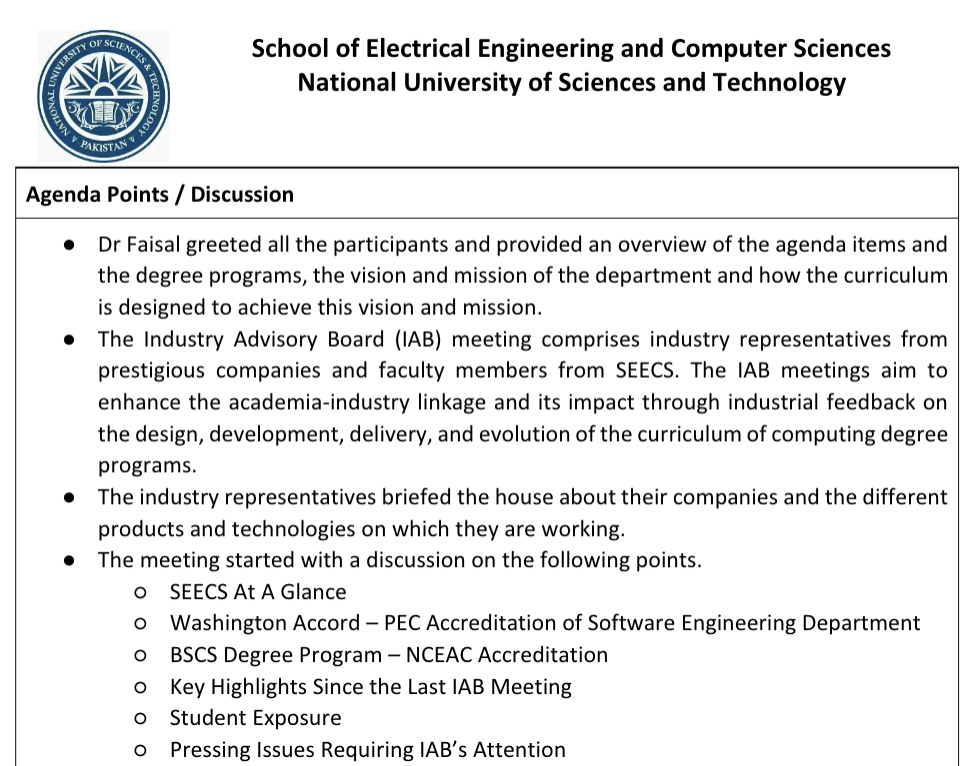
\includegraphics[width=0.79\textwidth]{appendices/criterion_1/iab 2024a.png}
\caption{IAB Meeting 2nd May 2024}
\label{fig:iab 2024a}
\end{figure}

\begin{figure}[!h]
\centering
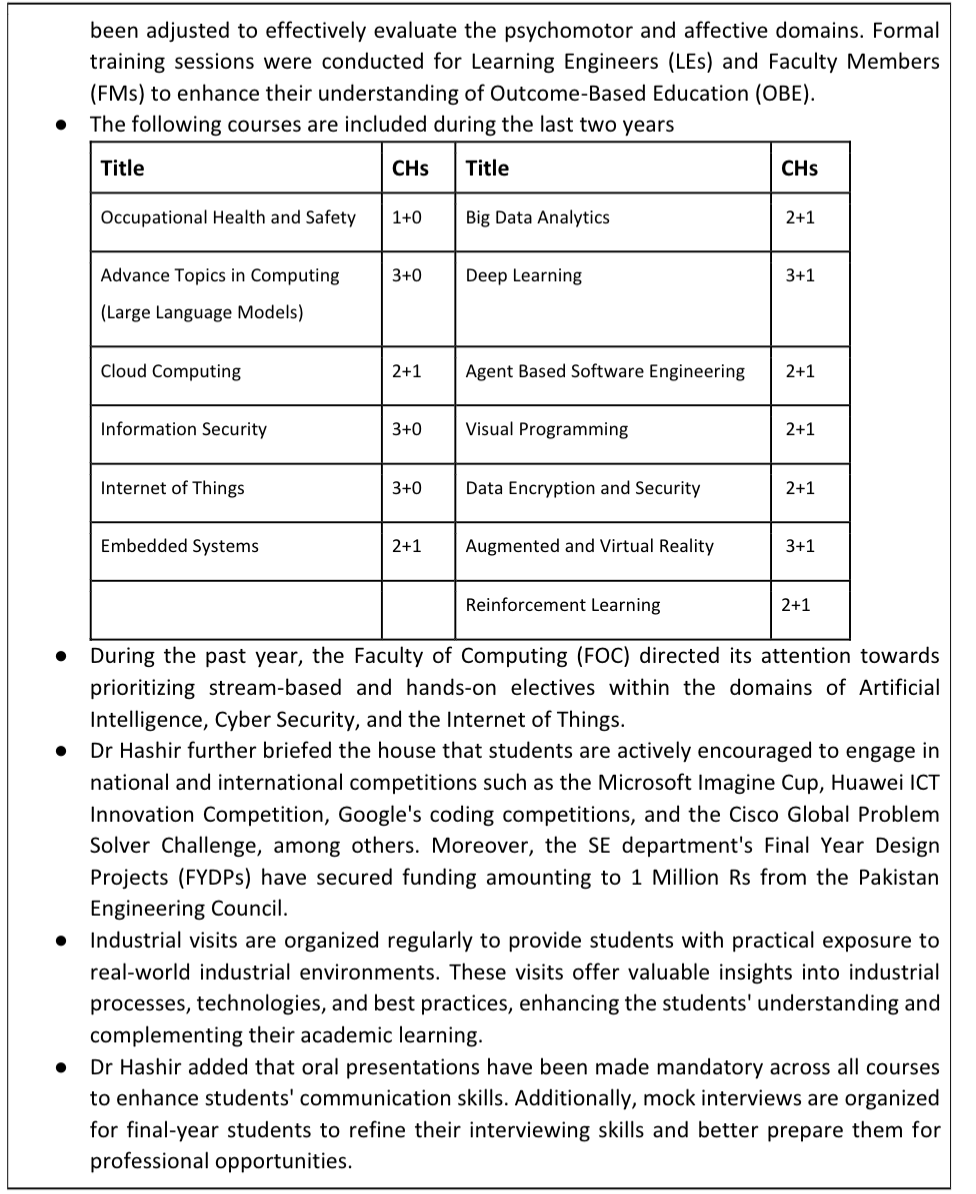
\includegraphics[width=0.85\textwidth]{appendices/criterion_1/iab 2024b.png}
\caption{IAB Meeting 2nd May 2024}
\label{fig:iab 2024b}
\end{figure}

Major participants included:

\begin{figure}[!h]
\centering
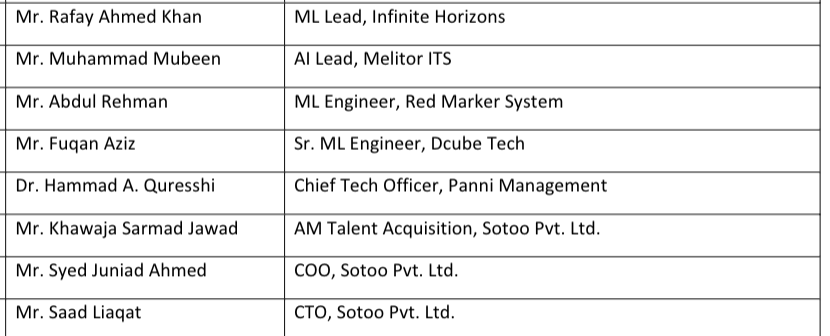
\includegraphics[width=0.75\textwidth]{appendices/criterion_1/iab 2024 attendees.png}
\caption{IAB Meeting Participants 2nd May 2024}
\label{fig:iab 2024 part}
\end{figure}

The next IAB meeting was held on 28th February 2025.

\begin{figure}[!h]
\centering
\fbox{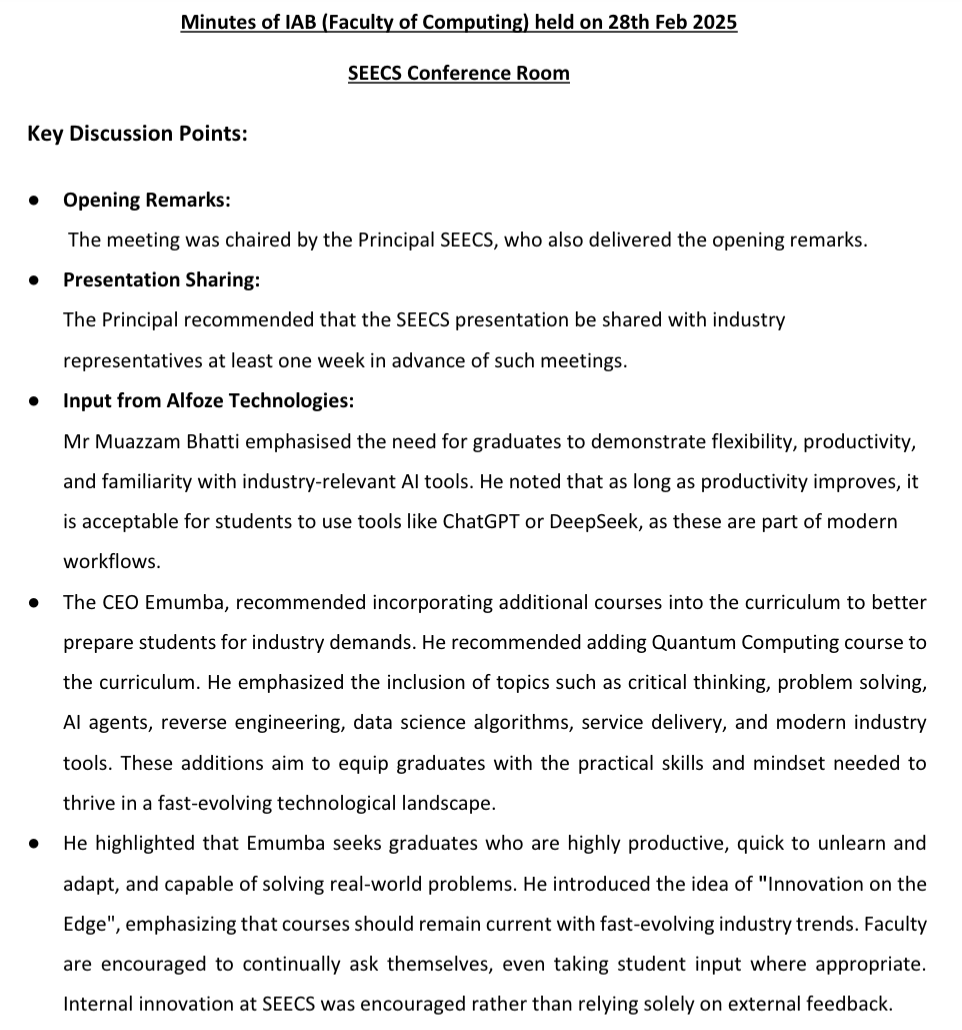
\includegraphics[width=0.80\textwidth]{appendices/criterion_1/iab 2025a.png}}
\caption{IAB Meeting 28th February 2025}
\label{fig:iab 2025a}
\end{figure}

\begin{figure}[!h]
\centering
\fbox{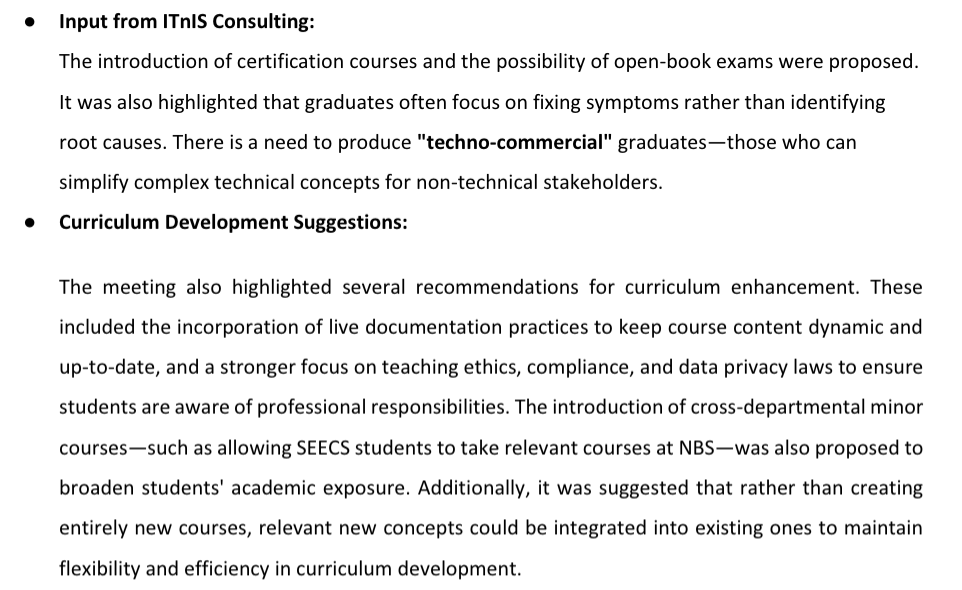
\includegraphics[width=0.80\textwidth]{appendices/criterion_1/iab 2025b.png}}
\caption{IAB Meeting 28th February 2025}
\label{fig:iab 2025b}
\end{figure}

The list of participants of the meeting is presented below:
\begin{figure}[!h]
\centering
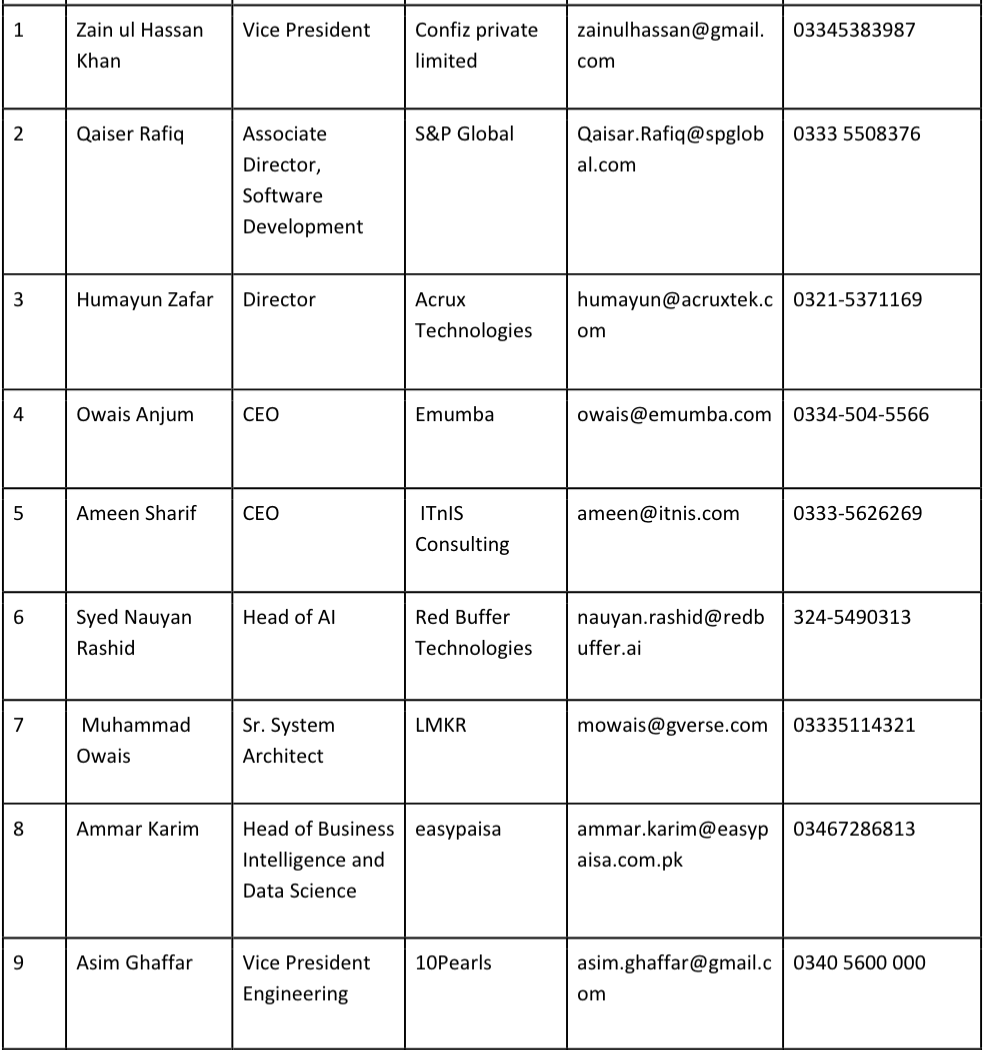
\includegraphics[width=0.75\textwidth]{appendices/criterion_1/iab 2025 attendees.png}
\caption{IAB Meeting Participants 28th February 2025}
\label{fig:iab 2025 attendees}
\end{figure}

The subsequent IAB meeting was held on 7th May 2025.

\begin{figure}[!h]
\centering
\fbox{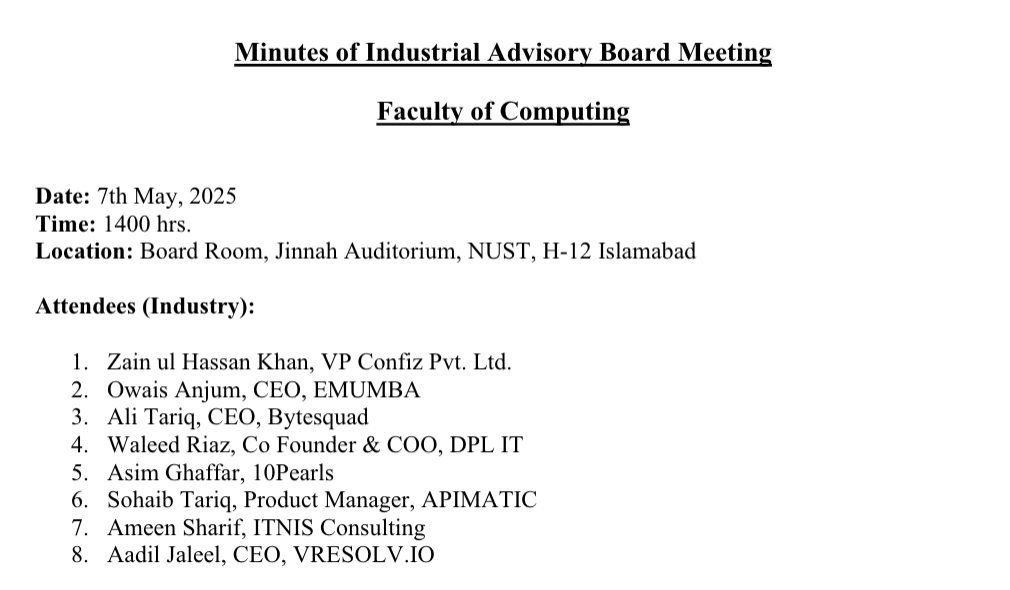
\includegraphics[width=0.80\textwidth]{appendices/criterion_1/iab 2025c.png}}
\caption{IAB Meeting Participants 7th May 2025}
\label{fig:iab 2025-2 attendees}
\end{figure}

\begin{figure}[!h]
\centering
\fbox{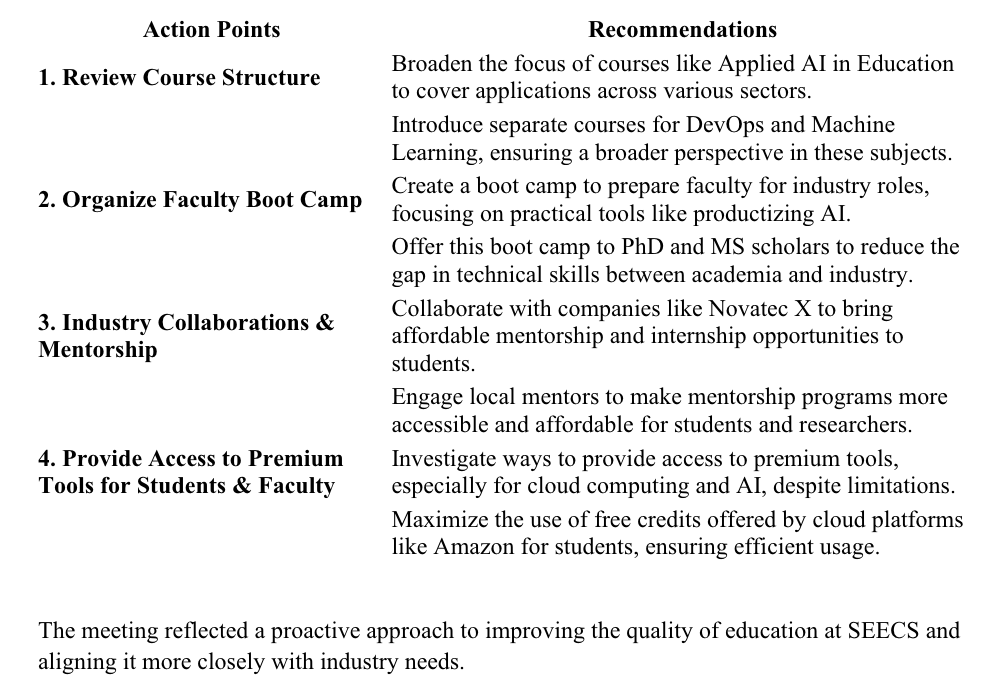
\includegraphics[width=0.85\textwidth]{appendices/criterion_1/iab 2025d.png}}
\caption{IAB Meeting 7th May 2025}
\label{fig:iab 2025d}
\end{figure}

The latest IAB meeting was held on 5th May 2026. The meeting was attended by following industry representatives:

\begin{figure}[!h]
\centering
\fbox{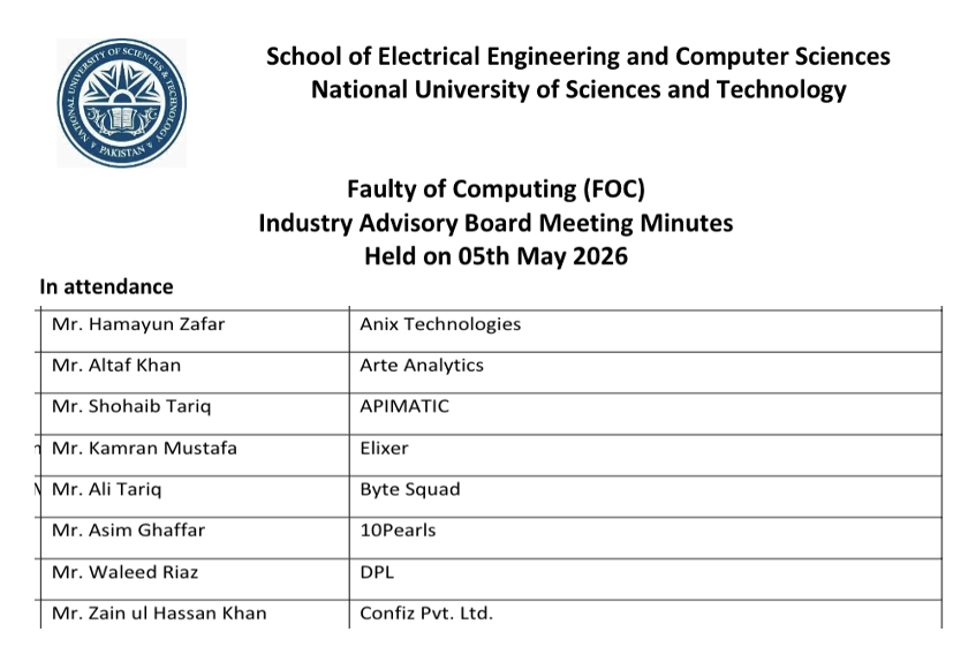
\includegraphics[width=0.85\textwidth]{appendices/criterion_1/iab 2026 attendees.png}}
\caption{IAB Meeting Participants 5th May 2026}
\label{fig:iab 2026 attendees}
\end{figure}

The main agenda points discussed in the meeting were following:

\begin{figure}[!ht]
\centering
\fbox{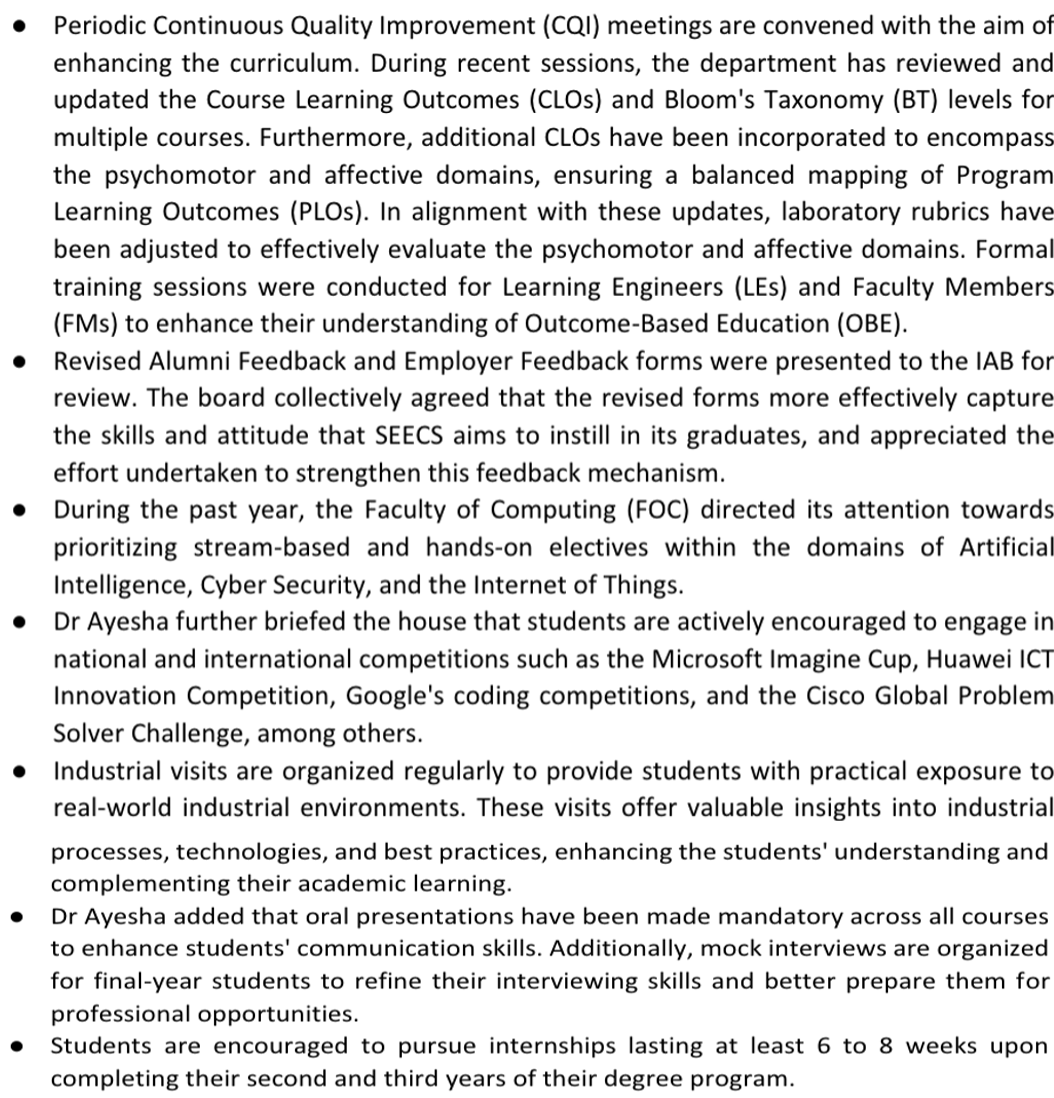
\includegraphics[width=0.85\textwidth]{appendices/criterion_1/iab 2026a.png}}
\caption{IAB Meeting 5th May 2026}
\label{fig:iab 2026a}
\end{figure}

\begin{figure}[!hb]
\centering
\fbox{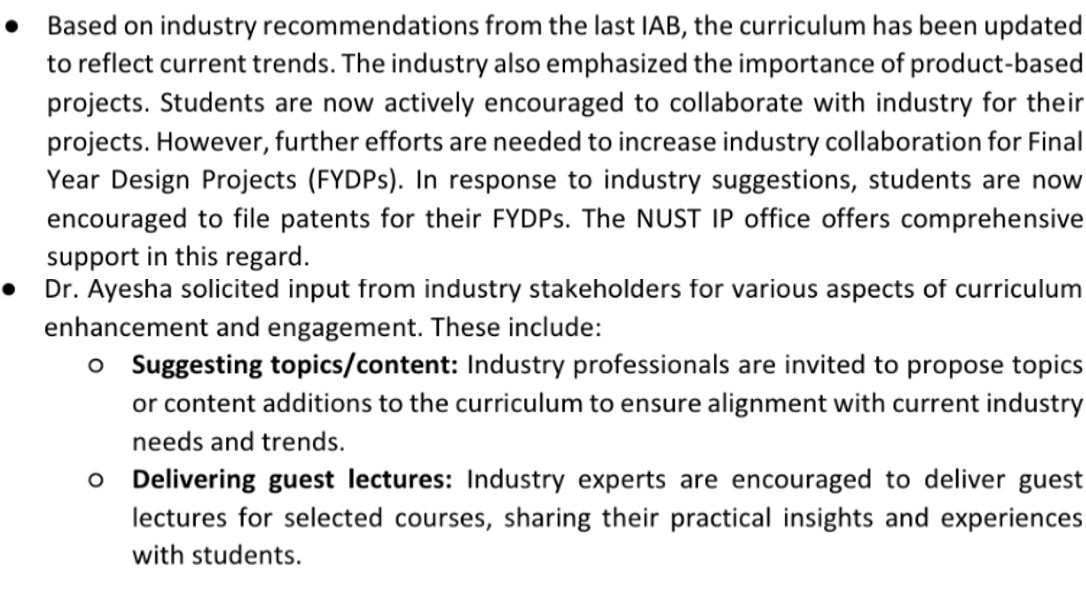
\includegraphics[width=0.85\textwidth]{appendices/criterion_1/iab 2026b1.png}}
\caption{IAB Meeting 5th May 2026}
\label{fig:iab 2026b1}
\end{figure}

\begin{figure}[!h]
\centering
\fbox{
\includegraphics[width=0.90\textwidth]{appendices/criterion_1/iab 2026c.png}}
\caption{IAB Meeting 5th May 2026}
\label{fig:iab 2026c}
\end{figure}

%Section~\ref{app:iab_feedback_full}. The 13th November 2023 session is retained below as the documented origin of the Revised (2026) PEO Evaluation System (Section~\ref{attainment-of-peos}).

%\subsection{IAB Meeting, 13th November 2023}
%The source file for this session also contains an appended briefing presentation (Annex-B) and PEO/KPI slides (Annex-C); consistent with the minutes-and-attendees-only scope of this section, only the two-page minutes and attendee list are reproduced below.
%\IfFileExists{appendices/criterion_1/IAB Meeting minutes - 13th Nov 2023.pdf}{%
%\begin{center}
%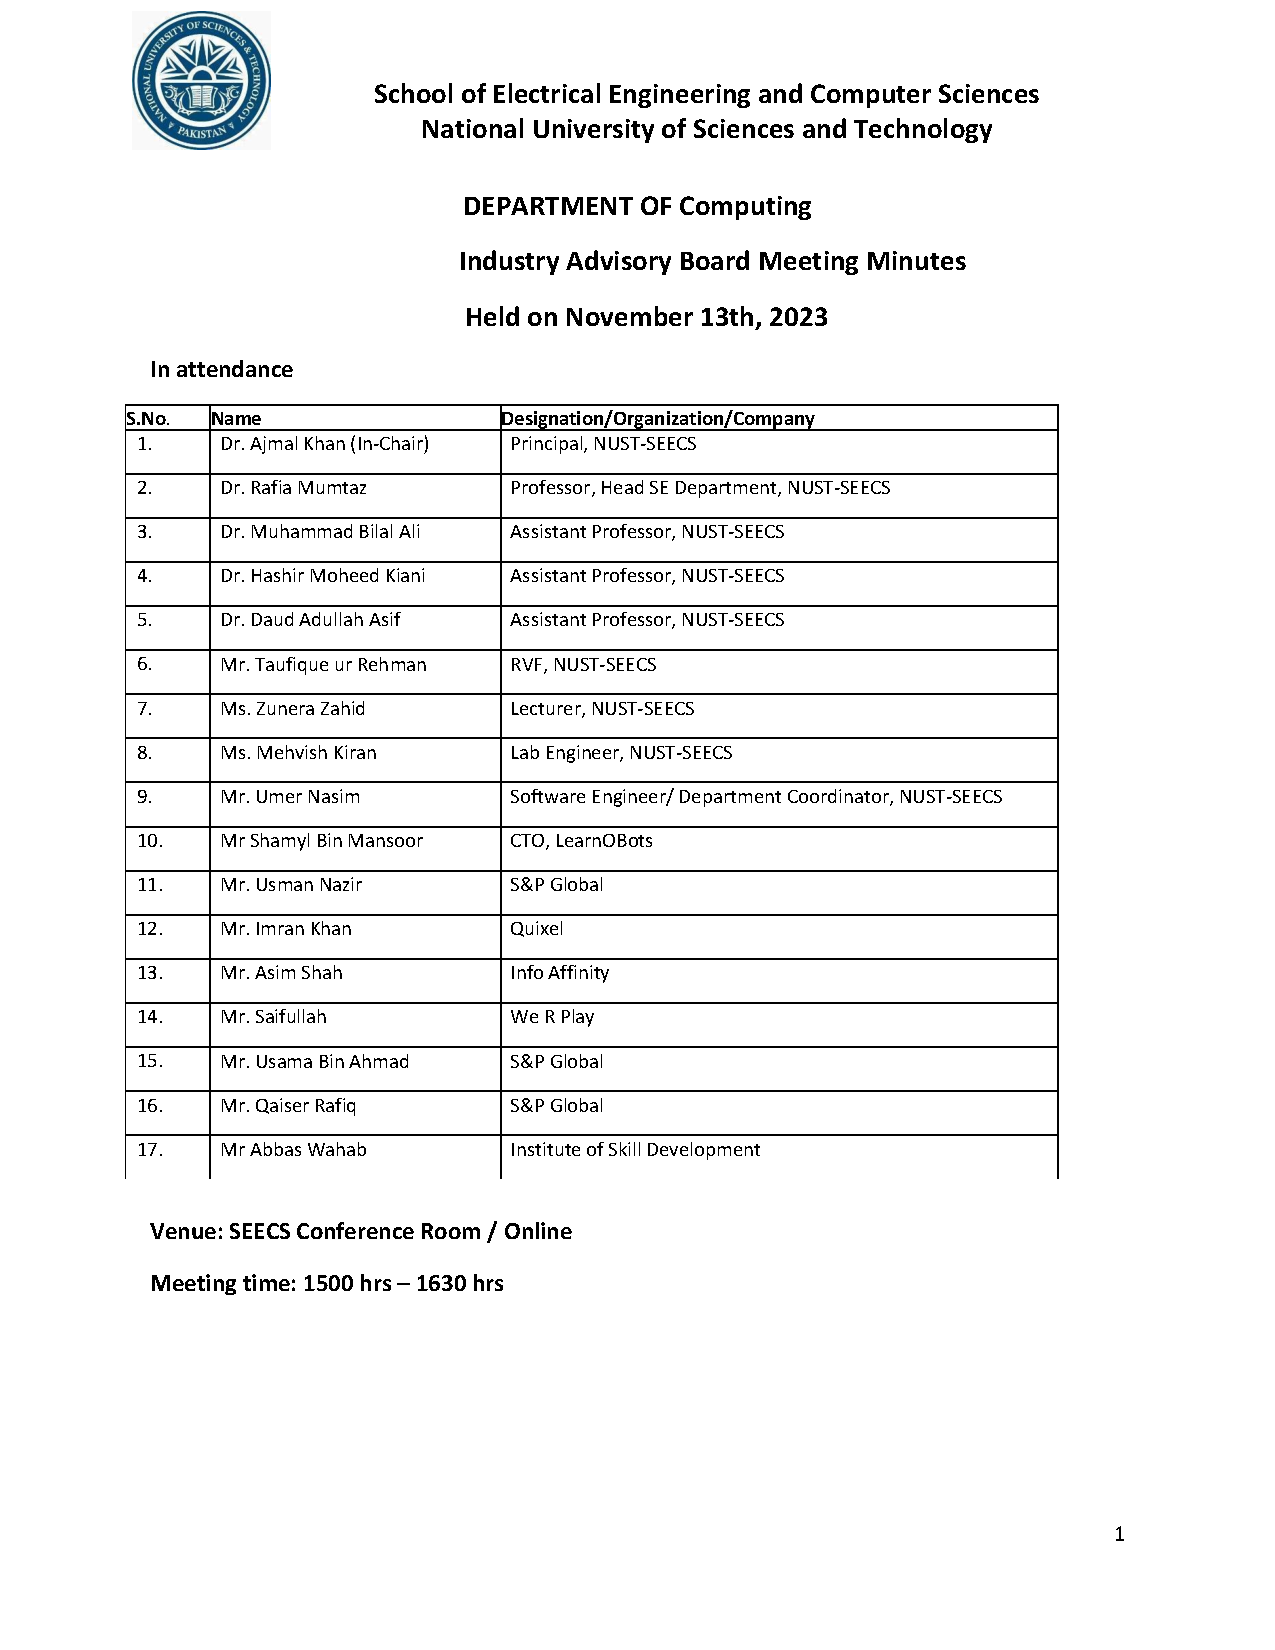
\includegraphics[page=1,width=0.92\textwidth]{appendices/criterion_1/IAB Meeting minutes - 13th Nov 2023.pdf}
%\end{center}
%\includepdf[pages=2]{appendices/criterion_1/IAB Meeting minutes - 13th Nov 2023.pdf}%
%}{\missingannexure{appendices/criterion_1/IAB Meeting minutes - 13th Nov 2023.pdf}}

%\subsection{IAB Meeting, 2nd May 2024}
%\includeminutesannexure{appendices/criterion_1/IAB Meeting minutes - 02nd May 2024.pdf}

%\subsection{IAB Meeting, 28th February 2025}
%\includeminutesannexure{appendices/criterion_1/IAB Meeting Minutes 28th Feb 2025.pdf}

%\subsection{IAB Meeting, 7th May 2025}
%\includeminutesannexure{appendices/criterion_1/IAB Meeting minutes 7th May 2025.pdf}

%\subsection{IAB Meeting, 5th May 2026}
%\includeminutesannexure{appendices/criterion_1/IAB_Meeting_minutes_05th_May_2026.pdf}

\section{Governance Minutes and Policy Documents }\label{app:governance_minutes}

This annexure presents the governance minutes and supporting policy documents cited in Criterion~1. Together, they provide documentary evidence that the Software Engineering programme operates within a formal, multi-level governance structure in which proposals are reviewed, approved and escalated through the appropriate academic bodies, and that stakeholder feedback is systematically acted upon. The annexure comprises the following documents:
\begin{itemize}
  \item Departmental Board of Studies (DBS) minutes, 20th April 2026.
  \item Faculty Board of Studies (FBS) minutes, 21st April 2026.
  \item Revised Internship Assessment Policy.
\end{itemize}

\begin{figure}[!h]
\centering
\fbox{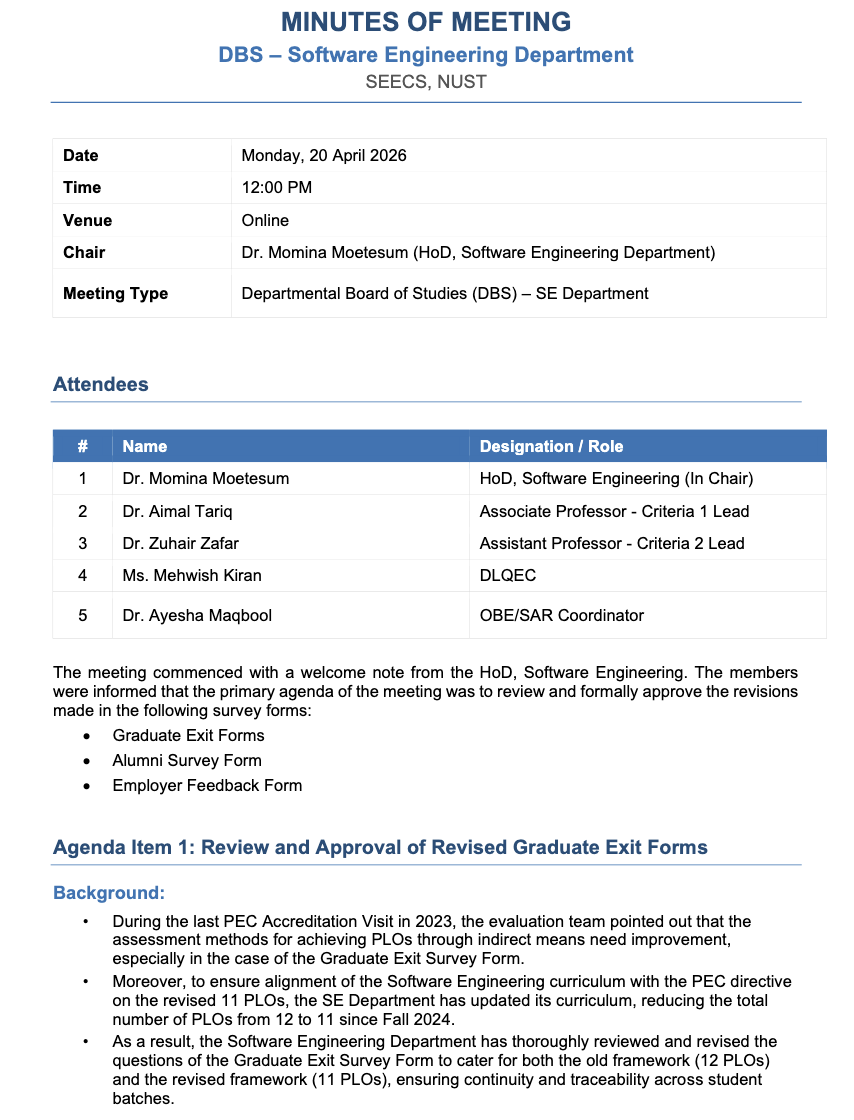
\includegraphics[width=1.0\textwidth]{appendices/criterion_1/dbs1.png}}
\caption{Department Board of Studies Meeting 20th April 2026}
\label{fig:dbs1}
\end{figure}

\begin{figure}[!h]
\centering
\fbox{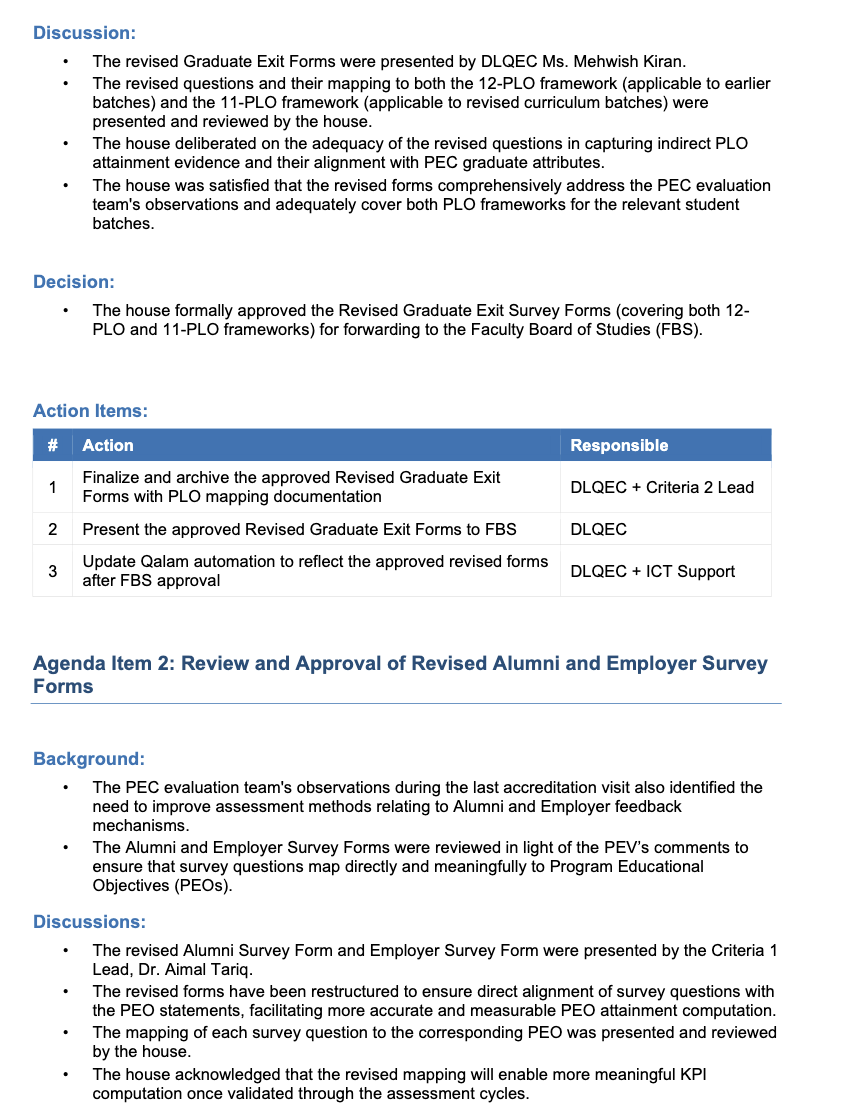
\includegraphics[width=1.0\textwidth]{appendices/criterion_1/dbs2.png}}
\caption{Department Board of Studies Meeting 20th April 2026}
\label{fig:dbs2}
\end{figure}

In addition, the DBS-approved working paper for the new elective course ``Introduction to Quantum Computing'', together with the proposal for the minor in Software Engineering, will be presented in detail in the
supporting evidence folder.

\begin{figure}[!h]
\centering
\fbox{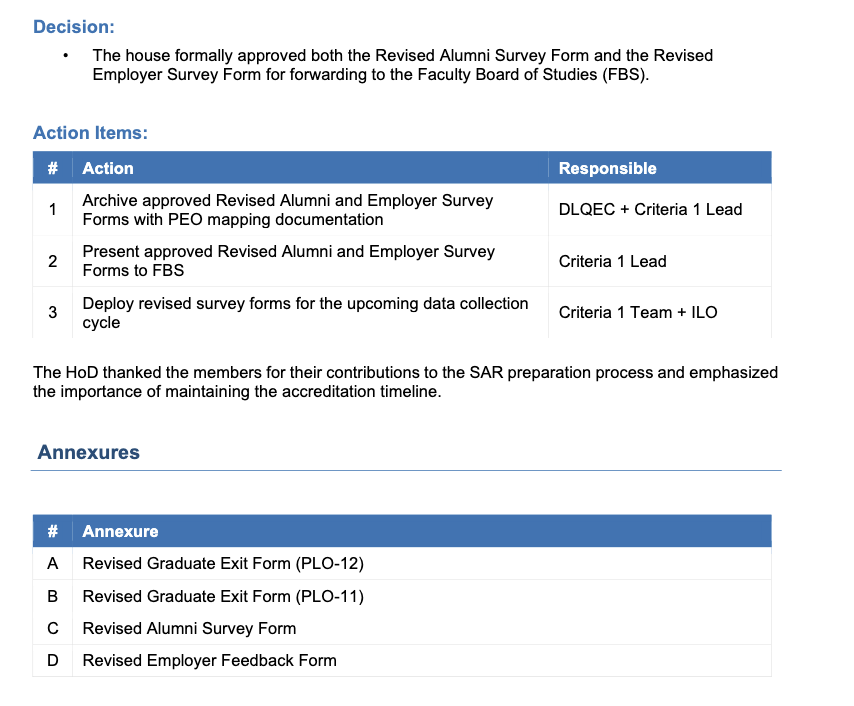
\includegraphics[width=0.75\textwidth]{appendices/criterion_1/dbs3.png}}
\caption{Department Board of Studies Meeting 20th April 2026}
\label{fig:dbs3}
\end{figure}

\begin{figure}[!h]
\centering
\fbox{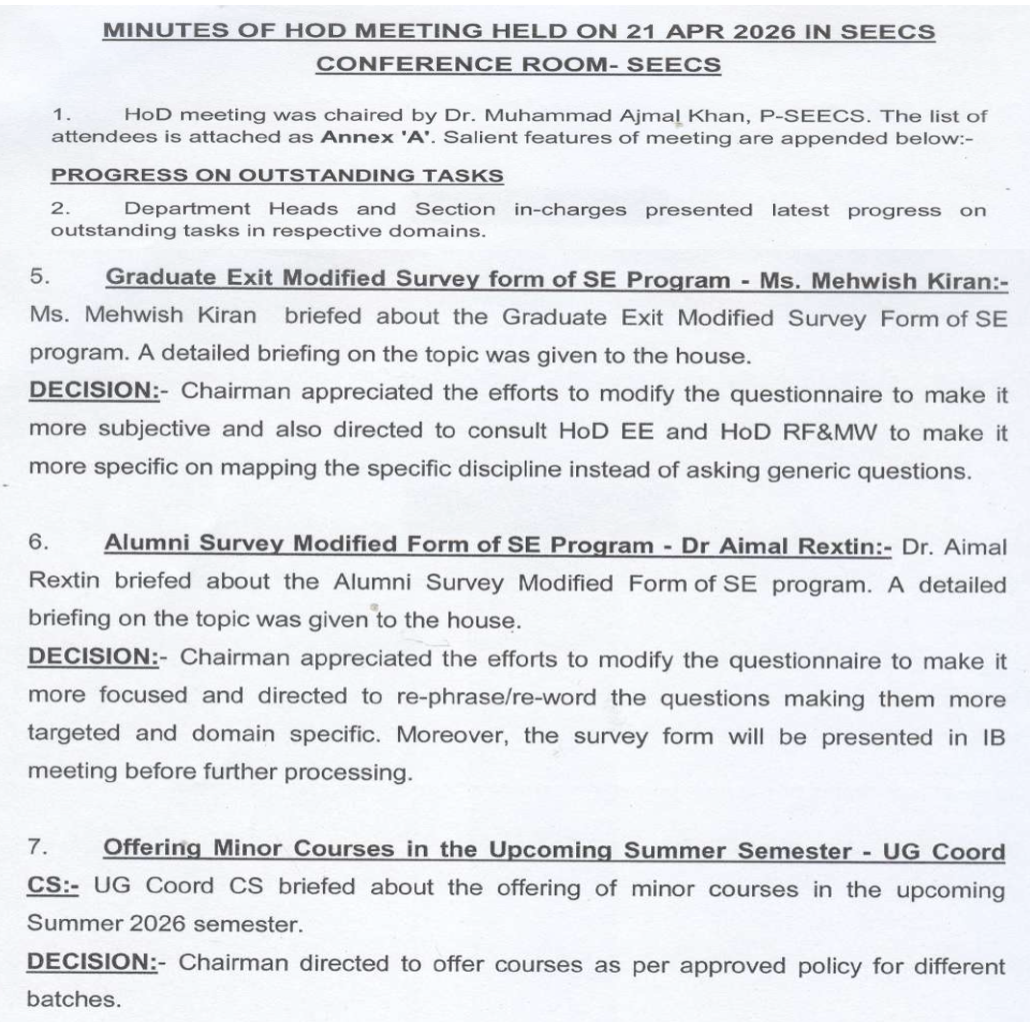
\includegraphics[width=0.75\textwidth]{appendices/criterion_1/fbs1.png}}
\caption{Faculty Board of Studies Meeting 21th April 2026}
\label{fig:fbs1}
\end{figure}

\begin{figure}[!h]
\centering
\fbox{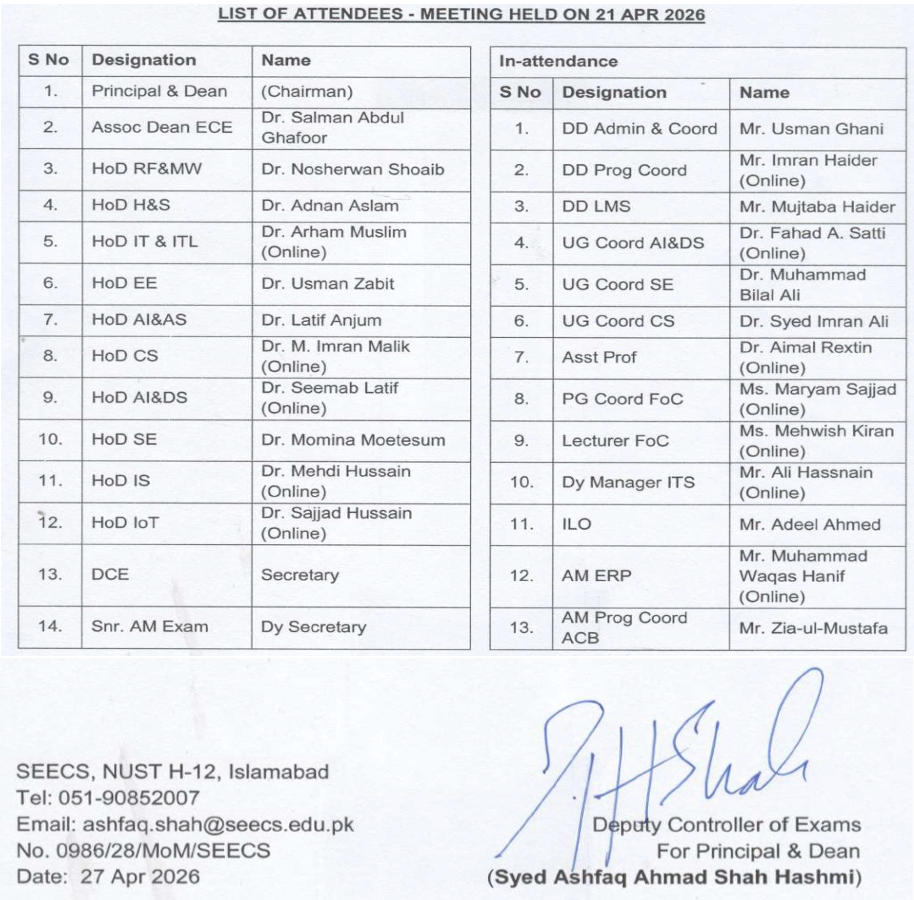
\includegraphics[width=0.80\textwidth]{appendices/criterion_1/fbs2.png}}
\caption{Faculty Board of Studies Meeting 20th April 2026}
\label{fig:fbs2}
\end{figure}

The internship policy defines the roles and responsibilities of the parties involved,
namely the student, the departmental internship supervisor and the industry supervisor at the host organisation. It specifies how student performance is evaluated, including the evaluation criteria, the weightage given to the industry supervisor's assessment and to the student's internship report, and the requirements for submitting documents. 
\begin{figure}[!h]
\centering
\fbox{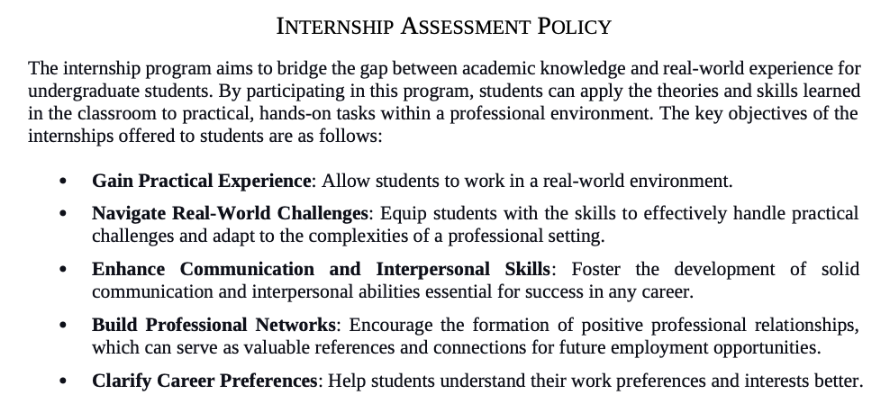
\includegraphics[width=0.80\textwidth]{appendices/criterion_1/internship1.png}}
\caption{Revised Internship Assessment Policy}
\label{fig:intern1}
\end{figure}

\begin{figure}[!h]
\centering
\fbox{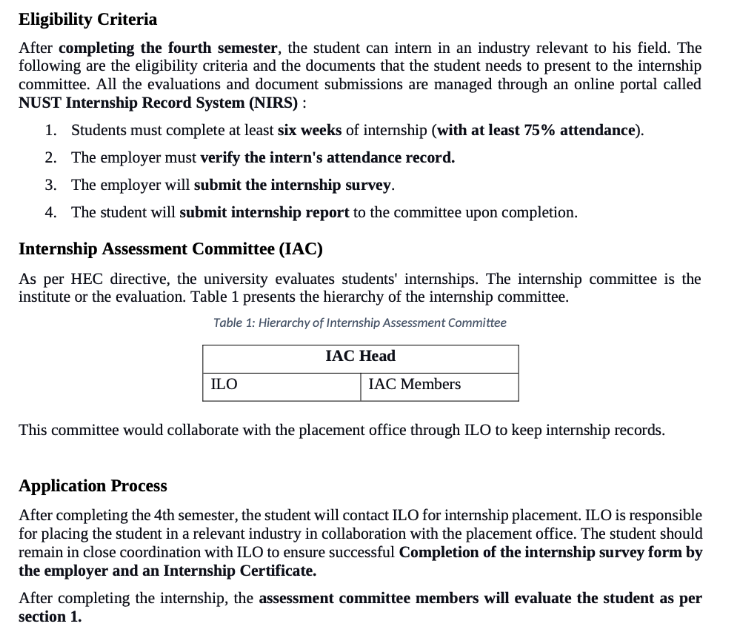
\includegraphics[width=0.80\textwidth]{appendices/criterion_1/internship1b.png}}
\caption{Revised Internship Assessment Policy}
\label{fig:intern1b}
\end{figure}

\begin{figure}[!h]
\centering
\fbox{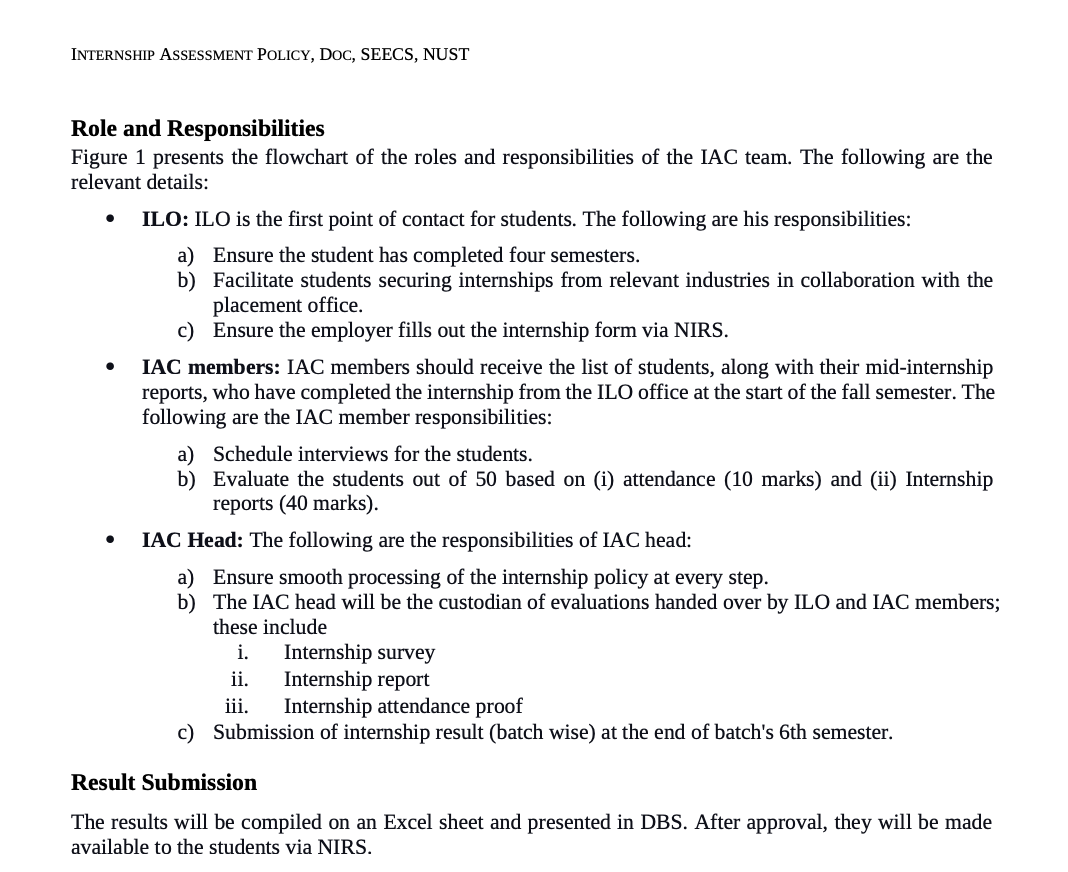
\includegraphics[width=0.80\textwidth]{appendices/criterion_1/internship2.png}}
\caption{Revised Internship Assesssment Policy}
\label{fig:intern2}
\end{figure}

\begin{figure}[!h]
\centering
\fbox{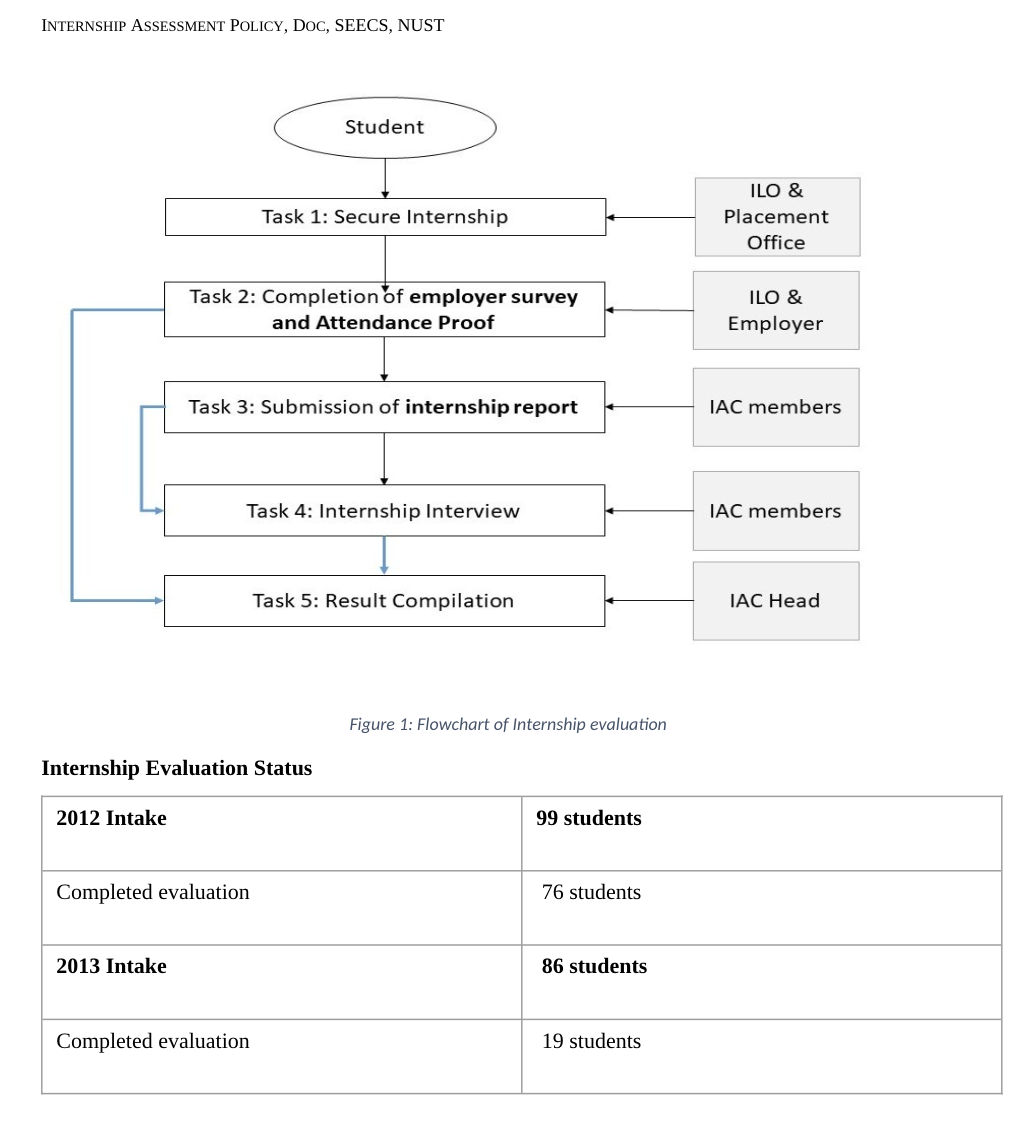
\includegraphics[width=0.80\textwidth]{appendices/criterion_1/internship3.png}}
\caption{Revised Internship Assessment Policy}
\label{fig:intern3}
\end{figure}

%\subsection{Internship Assessment Policy}
%\includefullannexure{appendices/criterion_1/Internship_Assessment_Procedure.pdf}

%\subsection{Minor in Software Engineering Offering in Spring 2026}
%\includefullannexure{appendices/criterion_1/Minors.pdf}

%%%%%%%%%%%%%%%%%%%%%%%%%%%%%%%%%%%
\newpage
\section{Revised Survey Forms}\label{app:revised forms}
The full Alumni and Employer Survey forms referenced in Criterion~1 are reproduced below exactly as administered, covering the revised (2026) evaluation system. These two instruments constitute the primary tools for the
indirect assessment of the Programme Educational Objectives (PEOs). The Alumni Survey captures graduates' views on how well the programme has prepared them
for their careers and continued professional growth, while the Employer Survey records the perspective of organisations that employ or supervise our
graduates on their technical competence, professional conduct and overall performance in the workplace.

\begin{figure}[!h]
\centering
\fbox{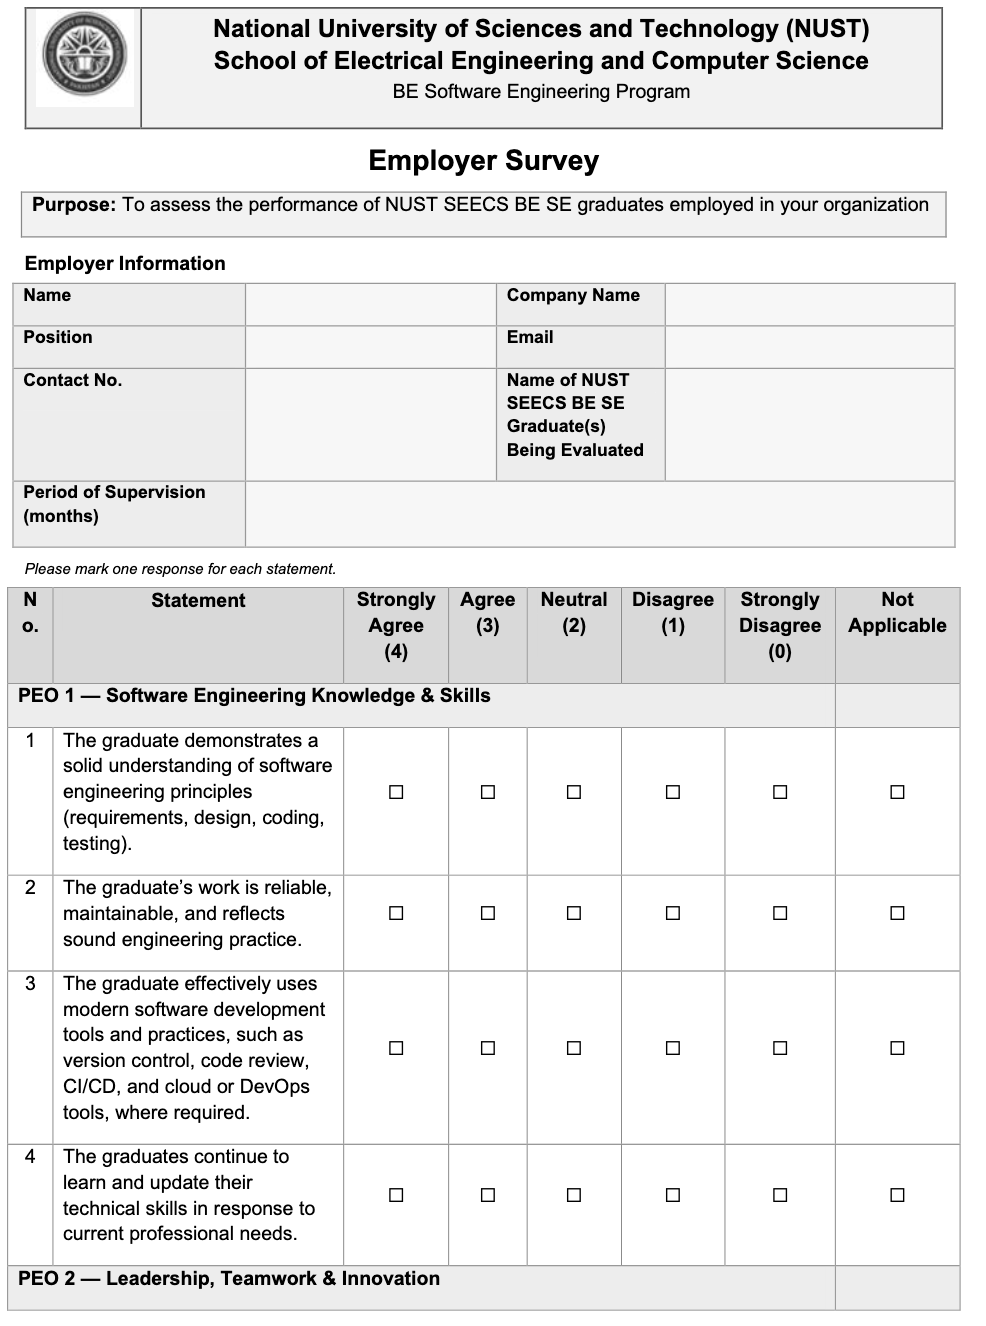
\includegraphics[width=1.0\textwidth]{appendices/criterion_1/revised employer form.png}}
\caption{Revised Employer Survey Form}
\label{fig:revised employer form}
\end{figure}

\begin{figure}[!h]
\centering
\fbox{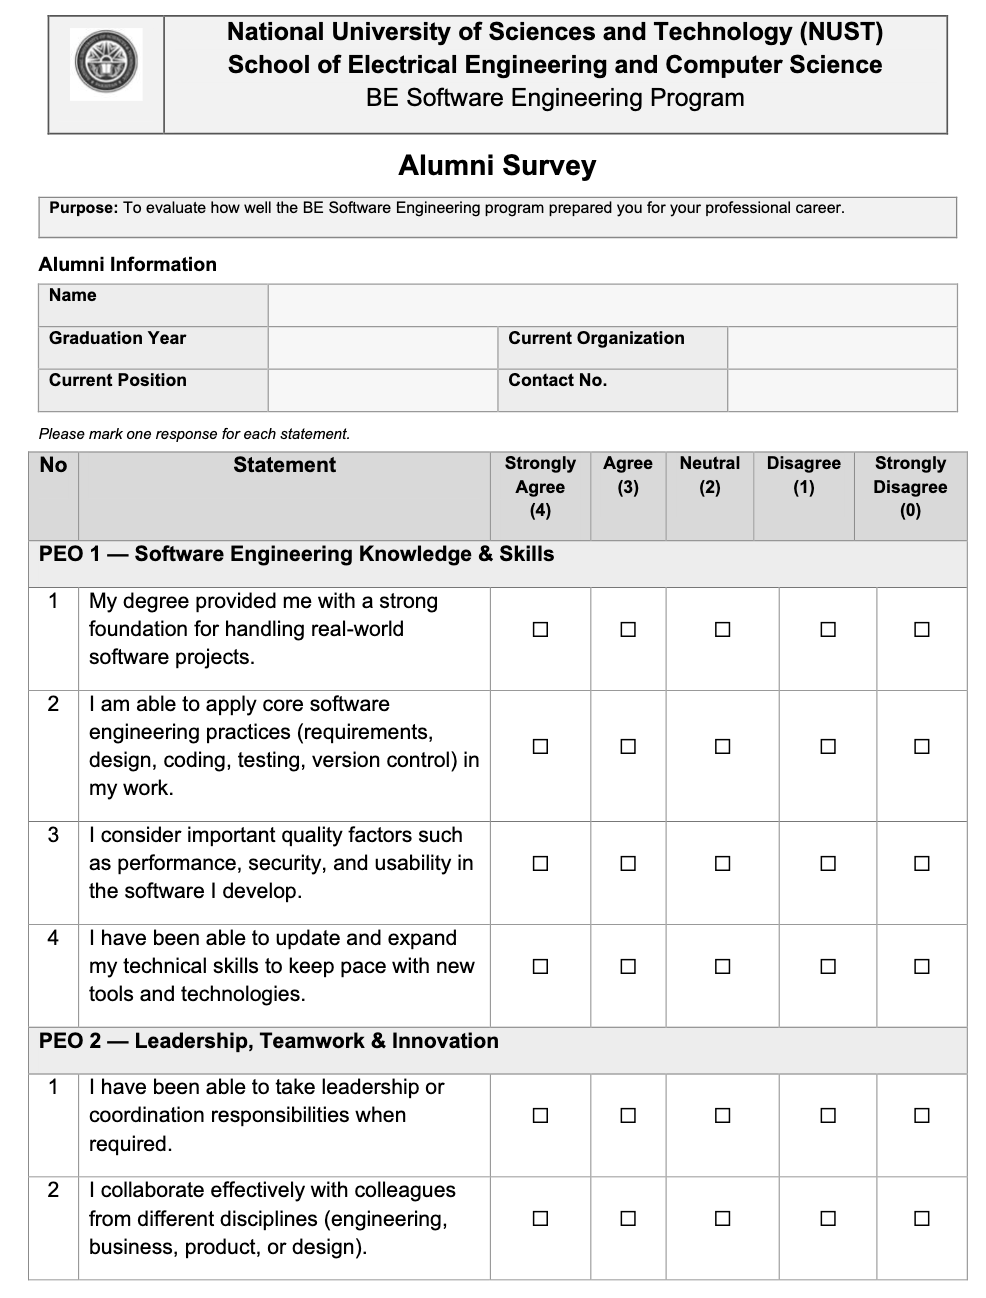
\includegraphics[width=1.0\textwidth]{appendices/criterion_1/revised alumni form.png}}
\caption{Revised Alumni Survey Form}
\label{fig:revised alumni form}
\end{figure}





%%%%%%%%%%%%%%%%%%%%%%%%%%%%%%%%%
%\section{Incorporation of Certifications in Degree Program}\label{app:certifications}

%This appendix highlights current directives from various governing bodies regarding inclusion/incorporation of certifications in degree programs. The Pakistan Engineering Council (PEC) (Letter PEC/EAD/EQEEP/2025/04, 14th July 2025)asked for institutional input on integrating international certifications into engineering programs in lieu of 6–12 credit hours of elective coursework. The Higher Education Commission (HEC) (Letter HEC/CURR/GEN/2025/8036, 15th September 2025) subsequently issued a formal advisory mandating incorporation of industry certifications and internships into undergraduate programs, with specific provision for CS/IT programs to replace electives with certifications equivalent to 3 credit hours. In response, NUST processed Working Paper No. 2 (73rd ACM, 9th February 2026), endorsed at UCAP on 30th January 2026, establishing a formal mechanism for certification credit-hour recognition (1–3 CH per certification, subject to CLO-mapping, department-level validation/assessment, and ACM approval), recommended for implementation with immediate effect. Each directive is presented as a separate section, with the source PDF embedded in full immediately below its heading.

%\subsection{Pakistan Engineering Council (PEC)'s Letter }
%\includefullannexure{appendices/criterion_1/PEC-Letter-Certifications.pdf}

%\subsection{Higher Education Commission (HEC)'s Letter}
%\includefullannexure{appendices/criterion_1/HEC-Certification.pdf}

%\subsection{NUST Working Paper}
%\includefullannexure{appendices/criterion_1/NUST-WP-Certification.pdf}

